% Copyright (C) 2014-2020 by Thomas Auzinger <thomas@auzinger.name>

\documentclass[draft,final]{vutinfth} % Remove option 'final' to obtain debug information.

% Load packages to allow in- and output of non-ASCII characters.
\usepackage{lmodern}        % Use an extension of the original Computer Modern font to minimize the use of bitmapped letters.
\usepackage[T1]{fontenc}    % Determines font encoding of the output. Font packages have to be included before this line.
\usepackage[utf8]{inputenc} % Determines encoding of the input. All input files have to use UTF8 encoding.
\usepackage[fontsize=12pt]{fontsize}
\usepackage[htt]{hyphenat}

% Extended LaTeX functionality is enables by including packages with \usepackage{...}.
\usepackage{amsmath}    % Extended typesetting of mathematical expression.
\usepackage{amssymb}    % Provides a multitude of mathematical symbols.
\usepackage{mathtools}  % Further extensions of mathematical typesetting.
\usepackage{microtype}  % Small-scale typographic enhancements.
\usepackage[inline]{enumitem} % User control over the layout of lists (itemize, enumerate, description).
\usepackage{multirow}   % Allows table elements to span several rows.
\usepackage{booktabs}   % Improves the typesettings of tables.
\usepackage{subcaption} % Allows the use of subfigures and enables their referencing.
\usepackage[ruled,linesnumbered,algochapter]{algorithm2e} % Enables the writing of pseudo code.
\usepackage[usenames,dvipsnames,table]{xcolor} % Allows the definition and use of colors. This package has to be included before tikz.
\usepackage{nag}       % Issues warnings when best practices in writing LaTeX documents are violated.
\usepackage{pdfpages}
\usepackage{todonotes} % Provides tooltip-like todo latex-tips.
\usepackage{hyperref}  % Enables cross linking in the electronic document version. This package has to be included second to last.
\usepackage[nameinlink]{cleveref}
\usepackage{listings}
\usepackage{tikz}
\usepackage[square, numbers, sort]{natbib}
\usepackage{lipsum} % Enables the generation of glossaries and lists fo acronyms. This package has to be included last.

\lstset{
    basicstyle=\footnotesize\ttfamily,        % the size of the fonts that are used for the code
    breakatwhitespace=false,         % sets if automatic breaks should only happen at whitespace
    breaklines=true,                 % sets automatic line breaking
    captionpos=b,                    % sets the caption-position to bottom
    commentstyle=\color{gray},    % comment style
    keywordstyle=\color[HTML]{A55C86},
    stringstyle=\color{green!50!black},
    showstringspaces=false,
    extendedchars=true,              % lets you use non-ASCII characters; for 8-bits encodings only, does
    keepspaces=true,                 % keeps spaces in text, useful for keeping indentation of code
    numbers=left,                    % where to put the line-numbers; possible values are (none, left, right)
    numbersep=5pt,                   % how far the line-numbers are from the code
    numberstyle=\tiny, % the style that is used for the line-numbers
    tabsize=4,                     % sets default tabsize to 2 spaces
    title=\lstname                   % show the filename of files included with \lstinputlisting; also
}

\lstdefinelanguage{Kotlin}{
    alsoletter={!},
    keywords=[1]{if, return, !in, fun, class, private, val, data, interface, null},
    keywordstyle=[1]\color[HTML]{761629}, % light-purple
    keywords=[2]{String, List, Sequence, T, String, CityController, City, Long, Double, CityMapService, GenerationType, Bounds, Pair},
    keywordstyle=[2]\color[HTML]{007E8A}, % light-blue
    keywords=[3]{list, first, tail, head, tailList, size, it, string, cityRepository, cityMapService, id, name, x, y, IDENTITY},
    keywordstyle=[3]\color[HTML]{7D3781}, % purple
    keywords=[4]{@RestController, @Entity, @Repository, @RequestMapping, @PostMapping, @GetMapping, @Transactional, @DeleteMapping,
    @RequestBody, @PathVariable, @Id, @GeneratedValue, @Column},
    keywordstyle=[4]\color[HTML]{9A892E}, % yellow
    keywords=[5]{CityRepository, JpaRepository},
    keywordstyle=[5]\color[HTML]{5E54AB}, % weird-blue
    morecomment=[l]{//}, % l is for line comment
    morecomment=[s]{/*}{*/}, % s is for start and end delimiter
    morestring=[b]", % defines that strings are enclosed in double quotes
    literate={0}{{\textcolor{blue}{0}}}{1}%
        {v1}{{\textcolor{green!50!black}{v1}}}{2}%
        {1}{{\textcolor{blue}{1}}}{1}%
        {2}{{\textcolor{blue}{2}}}{1}%
        {3}{{\textcolor{blue}{3}}}{1}%
        {4}{{\textcolor{blue}{4}}}{1}%
        {5}{{\textcolor{blue}{5}}}{1}%
        {6}{{\textcolor{blue}{6}}}{1}%
        {7}{{\textcolor{blue}{7}}}{1}%
        {8}{{\textcolor{blue}{8}}}{1}%
        {9}{{\textcolor{blue}{9}}}{1}%
        {.0}{{\textcolor{blue}{.0}}}{2}% Following is to ensure that only periods
        {.1}{{\textcolor{blue}{.1}}}{2}% followed by a digit are changed.
        {.2}{{\textcolor{blue}{.2}}}{2}%
        {.3}{{\textcolor{blue}{.3}}}{2}%
        {.4}{{\textcolor{blue}{.4}}}{2}%
        {.5}{{\textcolor{blue}{.5}}}{2}%
        {.6}{{\textcolor{blue}{.6}}}{2}%
        {.7}{{\textcolor{blue}{.7}}}{2}%
        {.8}{{\textcolor{blue}{.8}}}{2}%
        {.9}{{\textcolor{blue}{.9}}}{2}%
} %

\lstdefinelanguage{JavaScript}{
    keywords=[1]{if, return, this, else, import, from, export, class, const, new, function, null},
    keywordstyle=[1]\color[HTML]{761629}, % red
    keywords=[2]{List, Sequence, T, String, HomeComponent, Scene, PerspectiveCamera, WebGLRenderer, BoxGeometry, MeshBasicMaterial, Mesh},
    keywordstyle=[2]\color[HTML]{007E8A}, % light-blue
    keywords=[3]{list, first, tail, head, tailList, size, it, string, selector, templateUrl, styleUrls, window, innerWidth, innerHeight,
    position, scene, camera, renderer, geometry, material, cube, color, raycaster, selectedObject, intersection, length, object, castTargets, mouse},
    keywordstyle=[3]\color[HTML]{7D3781}, % purple
    keywords=[4]{@Component, setSize, add},
    keywordstyle=[4]\color[HTML]{9A892E}, % yellow
    morecomment=[l]{//}, % l is for line comment
    morecomment=[s]{/*}{*/}, % s is for start and end delimiter
    morestring=[b]', % defines that strings are enclosed in double quotes
    literate={0}{{\textcolor{blue}{0}}}{1}%
        {1}{{\textcolor{blue}{1}}}{1}%
        {2}{{\textcolor{blue}{2}}}{1}%
        {3}{{\textcolor{blue}{3}}}{1}%
        {4}{{\textcolor{blue}{4}}}{1}%
        {5}{{\textcolor{blue}{5}}}{1}%
        {6}{{\textcolor{blue}{6}}}{1}%
        {7}{{\textcolor{blue}{7}}}{1}%
        {8}{{\textcolor{blue}{8}}}{1}%
        {9}{{\textcolor{blue}{9}}}{1}%
        {0x00ff00}{{\textcolor{blue}{0x00ff00}}}{8}%
        {.0}{{\textcolor{blue}{.0}}}{2}% Following is to ensure that only periods
        {.1}{{\textcolor{blue}{.1}}}{2}% followed by a digit are changed.
        {.2}{{\textcolor{blue}{.2}}}{2}%
        {.3}{{\textcolor{blue}{.3}}}{2}%
        {.4}{{\textcolor{blue}{.4}}}{2}%
        {.5}{{\textcolor{blue}{.5}}}{2}%
        {.6}{{\textcolor{blue}{.6}}}{2}%
        {.7}{{\textcolor{blue}{.7}}}{2}%
        {.8}{{\textcolor{blue}{.8}}}{2}%
        {.9}{{\textcolor{blue}{.9}}}{2}%
} %

% Define convenience functions to use the author name and the thesis title in the PDF document properties.
\newcommand{\authorname}{Merjem Štulanović} % The author name without titles.
\newcommand{\thesistitle}{Capturing the Life of an Artist Using Information Visualization Techniques} % The title of the thesis. The English version should be used, if it exists.

% Set PDF document properties
\hypersetup{
    pdfpagelayout   = TwoPageRight,           % How the document is shown in PDF viewers (optional).
    linkbordercolor = {Melon},                % The color of the borders of boxes around crosslinks (optional).
    pdfauthor       = {\authorname},          % The author's name in the document properties (optional).
    pdftitle        = {\thesistitle},         % The document's title in the document properties (optional).
    pdfsubject      = {Subject},              % The document's subject in the document properties (optional).
    pdfkeywords     = {a, list, of, keywords} % The document's keywords in the document properties (optional).
}

\linespread{1.25}
\setpnumwidth{2.5em}        % Avoid overfull hboxes in the table of contents (see memoir manual).
\setsecnumdepth{subsection} % Enumerate subsections.

\nonzeroparskip             % Create space between paragraphs (optional).
\setlength{\parindent}{0pt} % Remove paragraph identation (optional).

%\glstocfalse   % Remove the glossaries from the table of contents.

% Set persons with 4 arguments:
%  {title before name}{name}{title after name}{gender}
%  where both titles are optional (i.e. can be given as empty brackets {}).
\setauthor{}{\authorname}{}{female}
\setadvisor{}{Fabio Pittarello}{}{male}

% Required data.
\setregnumber{882311}
\setdate{02}{11}{2021} % Set date with 3 arguments: {day}{month}{year}.
\settitle{\thesistitle}{\thesistitle} % Sets  the title. If your title contains commas, enclose it with additional curvy brackets (i.e., {{your title}}) or define it as a macro as done with \thesistitle.
\setsubtitle{}{} % Sets the subtitle. Use {} if none.

\setthesis{master}
\setmasterdegree{dipl.}

\setcurriculum{Data Management and Analytics}{} % Sets the English and German name of the curriculum.

\begin{document}

    \frontmatter % Switches to roman numbering.
% The structure of the thesis has to conform to the guidelines at
%  https://informatics.tuwien.ac.at/study-services

    %\addtitlepage{english} % English title page.

    \includepdf[pages=-]{content/front-page.pdf}

%    \addstatementpage

    \begin{acknowledgements*}
        A number of people helped me throughout these years of my masters education at
        Ca' Foscari University of Venice. Starting from professors who were always delivering
        their knowledge in the best possible way, lecturers, and administrative staff at the University,
        I would like to thank everyone who played some role in my education during these years.
        The Computer Science Department is for sure one of the best at the University,
        and it met all of my expectations.

        I express my sincere gratitude to my mentor Prof. Fabio Pittarello for being
        supportive, patient, and helpful during this time. He played a significant role in
        delivering the thesis in the best possible way.

        I cannot forget to thank all of my friends and colleagues that were here with me
        during my studies. We had a lot of fun and created some beautiful memories
        which will be cherished forever. Their friendship is one of the most important things
        I will take with me while leaving these doors behind me.

        The last words of thanks go to my family and people who helped me in any kind of
        way during my education. If it were not for them, I would not have been able to accomplish
        all of this. Their unselfish support was present all the time and helped me in the
        toughest moments. I hope I get to return all of this to them one day.
    \end{acknowledgements*}

    \begin{abstract}
        Visualizing information correctly and in a useful way is a difficult task in computer science. Information is
        collected from many subject fields, and presenting it purposefully can often be challenging for a scientist or
        a researcher. Not only does one have to transform the raw data into something more comprehensible, but do it
        in a way that makes concepts more familiar. One of the most important tasks that need to be
        fulfilled is presenting data in a proper way, compliant with the users' background and skills, in
        order to permit them to form a mental model of the subject.

        The subject field of this master's thesis is art, specifically artists and their lives, investigated through
        computer science. This research will try to capture the life of an artist using specific information
        visualization techniques, even enhancing the already seen ones to adjust them to this special subject field. It will
        focus on spatio-temporal visualization techniques, adapting them to the art field, and in the end, implementing
        all research work into an augmented reality prototype. The goal is to combine computer science and arts by
        presenting users, like art experts, visitors of an art exhibition or a museum, with an innovative way of learning about the
        life of an artist, summarizing the most important parts of their lives with meaningful and interactive information
        visualization techniques.
    \end{abstract}

% Select the language of the thesis.
    \selectlanguage{english}

% Add a table of contents (toc).
    \setcounter{tocdepth}{4}
    \tableofcontents % Starred version, i.e., \tableofcontents*, removes the self-entry.

% Switch to arabic numbering and start the enumeration of chapters in the table of content.
    \mainmatter

    \chapter{Introduction}\label{ch:introduction}
    In this chapter, we will talk about the conceptual development and implementation part of the thesis. As previously said, the space-time cube was chosen to present
artists' lives. Several technologies were used in order to implement this visualization, more about them was mentioned in \Cref{ch:background}.

The original concept of the space-time cube along with the examples we have seen was just the starting point of creating the visualization. It was
necessary to decide which parts of their lives to include in the cube. Also, it was necessary to decide which external events to integrate in it,
to make the visualization more meaningful. Additional information was included, like exhibitions artists attended, important stays in their life,
minor/major historical events that might have influenced artists' lives, connections between multiple artists, and others. These were combined
with the space-time path that represents the artists' movement during their life. Each of these parameters will be explained in detail and the
most important and interesting examples of the code will be mentioned.

\clearpage

Before presenting the implementation aspects of the representation of the space-time cube, we present parameters and features that were selected for the representation in the cube:
\begin{itemize}
    \item The first feature represents the space-time path of an artist's life. The path will show the activity during their life. This trajectory will include locations of their stays and the length of each stay. Some stays could be important for different reasons, because of this, they will be specially marked. The choice of this feature was rather obvious, because visualizing a movement path is the primary purpose of a space-time cube.
    \item The second feature is related to the artistic part of an artist's life. This includes the artworks they created during their life. During our literature review, we saw representations that only concentrated on the artist's work, but did not include information on the life. Adding this feature to the space-time path combines multiple different representations into a single one.
    \item The third important feature which will be included are connections between artists. We saw examples of representations that show connections and relations between people, so including this aspect of an artist's life in the same visualization allows us to explore multiple space-time paths and examine the potential connections and relations between artists.
    \item The fourth feature we decided to represent are the exhibitions. These play important part in the artists' lives because they reflect on events attended by multiple artists and can help art experts to determine faster which artists were connected by mutual exhibitions.
    \item The last feature that we decided to implement are records of historic events which might have influenced artists' lives. These will not be related to artists closely, but will be included in the visualization independently. By observing these events, users will be able to see if some of them influenced the artists' life paths, for example, caused them to move elsewhere.
\end{itemize}

Since this is a 3D visualization and the AR part is animated through a mobile device, only the screenshots of the visualization will be
included in this chapter.
    \clearpage
    \section{Motivation and Goals}\label{sec:motivation-goals}
Visualization of cultural heritage has become recently popular thanks to the development of technology. We used to experience art collections
in person and in places where they are stored, such as museums, galleries, libraries, and archives~\citep{windhager2018visualization}. All
these artworks are visited and observed by people all around the world, with the spotlight being more oriented to the artworks rather than the artists
themselves. In order to understand the background of artists’ artworks and get an insight into their thinking, we need to explore their lives
too. For this reason, in addition to the visualization of artwork collections, it is useful to devote our attention and research to the
visualization of an artist’s life.

Information about the life of an artist is commonly presented in written form. We have biography books and memoirs~\citep{herrera1983frida,
    isaacson2017leonardo, tomkins1999duchamp}, articles, interviews, and others. The problem arises when we want to visualize their life
because there are many aspects and dimensions which can be taken into consideration and presented visually. Too much information may take over
the main goal of any information visualization -- transforming data into something more meaningful and easier to understand.

This research aims to visualize an artist’s life and provide a better understanding of the chosen dimensions, where the main goal is to
visually present their changes through space and time. The aim is to have a better understanding of artists' lives, to focus on undetected facts
and relations which may have influenced their works.

Here, we list the goals we want to accomplish during this research:

\begin{itemize}
    \item Visualize an artist's life path and places they lived in during their lifetime.
    \item Include the possibility to visualize multiple artists' lives and try to capture connections and interaction points, if any.
    \item Provide an interface for entering information about the artist’s life. In this way, the advanced users have complete control over the
            visualization and can create representations that are not available, without relying on third parties.
    \item Explore relevant events the artists might have attended, such as exhibitions that might have influenced their artistic production.
    \item Explore the minor or major historical events that may have influenced their lives and works.
    \item Make the visualization interactive with the possibility for the user/expert to filter the visualization parameters in order to
            focus on specific information.
    \item Combine the visualization with an augmented reality (AR) prototype for an immersive experience.
\end{itemize}

At this point, we would like to briefly explain the novelty of our work. During the research of literature, no examples of interactive space-time cubes that
combine artists' life paths with other aspects such as their work, attended events, etc. were found. Many of the works we surveyed focus on presenting a
single artist, whilst in our visualization, we allow the user to explore multiple lives and examine potential relations among artists. Additionally, none
of the works that we have seen provided manual insertion of data, but our work in contrast provides an easy-to-use interface that allows domain experts to
enter data themselves.

Lastly, we intend to make the first steps in interactive visualization of artists' lives, and present a clean implementation that will serve as
a foundation for further improvements and addition of new features. Based on our results, we hope to encourage research of the spatio-temporal
visualizations, especially in combination with the augmented reality experience.

    \section{Problem Statement}\label{sec:problem-statement}
The lack of visualizations for investigating artists’ lives is the problem this research will try to deal with and strive to provide a potential
solution to. Even though the information about how artists lived, worked, and everything else has been available in written form, aggregating and
converting that raw data into a visual representation has not been explored much. Partly because of the difficulty of putting one's life in
a comprehensive representation.

Humans are complex creatures and their lives are full of situations and experiences that shape them or change their life course. We need to
address the ones which crossed the life of an artist and present them in a meaningful way in this thesis. The purpose of this work is to improve the
previously seen space-time cube visualization and implement it as an augmented reality prototype. The space-time cube provides a great
foundation for presenting a person’s life, since its three dimensions allow for an exploration of both spatial and temporal properties.
    \section{Methodology and Solution Approach}\label{sec:methodology-solution-approach}
This section will cover the methodology and solution approach of the thesis research. We can divide our work into two parts, a literature
review of the previous works related to the thesis, and an implementation part based on the gathered knowledge.

In the literature review, we start from the early examples of information visualization and gradually present several categories like temporal,
geospatial, and spatio-temporal visualizations before we explore the one which will be used in our implementation, the space-time cube. We
address its points of strength and weakness, evaluations conducted on it, and see its applications in the cultural heritage domain. Another
important part of the literature review is related to the research on an artist’s life and the ways it is presented. This part helps us in
understanding which aspects of artists' lives are important to visualize and which visualizations help us do that in the best possible way.

For the implementation, several technologies were chosen to visualize the space-time cube. Angular, Three.js, and WebXR were used for the
frontend part, and the Spring Framework for the backend part. A web application is created that generates the space-time cube from the given data
inputs. An authoring interface is added that enables users/experts to enter their data into the application. In this way, the user is in control
of the system and can insert, edit or delete the data as they see fit, rather than relying on data provided by third parties. The interface can
manage artists and properties related to artists' lives, can filter information to present in the cube, and much more. The users can explore the
visualization in their browser or visualize the augmented reality version of the cube. This approach enhances 3D visualizations based on web
browsers, providing an additional engaging opportunities for exploring an artist's life.

For the evaluation of our work and results, we designed a pilot study proposal for around ten participants. It is composed of several
categories of questions related to the engagement (user's ability to effectively operate the visualization), learning (what knowledge was gained
through the interaction with the visualization), and general questions and comments (these include users' evaluation of the features and
feedback on which ones were well-received and where improvements could be made).

    \section{Structure}\label{sec:structure}
The structure of the work is divided into six chapters. \Cref{ch:literature-review} presents previous work and research in
information visualization, especially related to cultural heritage and the artists' lives. \Cref{ch:implementation} covers all the
work we have done in our implementation, describes the web application, how to use it, shows examples of it, and everything else
related to the prototype. \Cref{ch:background} briefly covers the technologies used for the implementation and gives insight into how and where
can we use them. \Cref{ch:evaluation} gives an evaluation of the visualization. In the last chapter, \Cref{ch:conclusion}, we conclude and sum up
what was done and mention future work plans.


    \chapter{Literature Review}\label{ch:literature-review}
    In this chapter, we will talk about the conceptual development and implementation part of the thesis. As previously said, the space-time cube was chosen to present
artists' lives. Several technologies were used in order to implement this visualization, more about them was mentioned in \Cref{ch:background}.

The original concept of the space-time cube along with the examples we have seen was just the starting point of creating the visualization. It was
necessary to decide which parts of their lives to include in the cube. Also, it was necessary to decide which external events to integrate in it,
to make the visualization more meaningful. Additional information was included, like exhibitions artists attended, important stays in their life,
minor/major historical events that might have influenced artists' lives, connections between multiple artists, and others. These were combined
with the space-time path that represents the artists' movement during their life. Each of these parameters will be explained in detail and the
most important and interesting examples of the code will be mentioned.

\clearpage

Before presenting the implementation aspects of the representation of the space-time cube, we present parameters and features that were selected for the representation in the cube:
\begin{itemize}
    \item The first feature represents the space-time path of an artist's life. The path will show the activity during their life. This trajectory will include locations of their stays and the length of each stay. Some stays could be important for different reasons, because of this, they will be specially marked. The choice of this feature was rather obvious, because visualizing a movement path is the primary purpose of a space-time cube.
    \item The second feature is related to the artistic part of an artist's life. This includes the artworks they created during their life. During our literature review, we saw representations that only concentrated on the artist's work, but did not include information on the life. Adding this feature to the space-time path combines multiple different representations into a single one.
    \item The third important feature which will be included are connections between artists. We saw examples of representations that show connections and relations between people, so including this aspect of an artist's life in the same visualization allows us to explore multiple space-time paths and examine the potential connections and relations between artists.
    \item The fourth feature we decided to represent are the exhibitions. These play important part in the artists' lives because they reflect on events attended by multiple artists and can help art experts to determine faster which artists were connected by mutual exhibitions.
    \item The last feature that we decided to implement are records of historic events which might have influenced artists' lives. These will not be related to artists closely, but will be included in the visualization independently. By observing these events, users will be able to see if some of them influenced the artists' life paths, for example, caused them to move elsewhere.
\end{itemize}

Since this is a 3D visualization and the AR part is animated through a mobile device, only the screenshots of the visualization will be
included in this chapter.
    \clearpage

\section{Brief History of Information Visualization}\label{sec:history-information-visualization}

%See \Cref{sec:information-visualization} for information about how we do this.
We use information visualization techniques to present data visually so that it is easier for people to understand it.
Throughout history, various ways of representing all kinds of data have been tried and developed. Some of the most
important and most used ones include tables, pie charts, bar charts, histograms, box and whisker plots, scatter plots, etc.

The first documented instance of a graph of statistical data is a 1644 graph by Michael Florent van Langren~\citep{friendly2010first}.
This one-dimensional line graph represents the twelve estimations of the difference in longitude between Toledo and
Rome and the names of astronomers who made the estimation.

\begin{figure}[h]
    \begin{center}
        % Vidiš ovo 0.5\textwidth je postotak širine stranice. ili samo \textwidth ako ćeš čitavom širinom
        %\includegraphics[width=0.5\textwidth]{graphics/1}
        %\includegraphics[width=2cm]{graphics/1}
        \includegraphics[width=\textwidth]{graphics/2-literature-review/1}
    \end{center}
    \caption{van Langren's 1644 graph of longitudes between Toledo and Rome~\citep{friendly2010first}}
    \label{fig:figure2.1}
\end{figure}

Other two important examples in the history of data visualization from the 19th century are Napoleon’s March Map
by Charles Joseph Minard and the Broad  Street Cholera Outbreak Map by John Snow. Napoleon’s March Map was described as
potentially the best statistical graphic ever drawn~\citep{tufte2001visual}.

The map shown in~\Cref{fig:figure2.2}, called the Sankey diagram nowadays, shows Napoleon’s huge losses during
his invasion of Russia in 1812. The army counted 422,000 soldiers at the beginning of the march, as indicated by the
thickness of the beige line, and managed to enter Russia with only 100,000 of them. The return to Poland was even more
disastrous, as shown by the lower black band, where most of the soldiers froze because of the cold winter. Only 10,000
men returned. Besides the army’s size and temperature, the map also shows its locations and movement direction.

\clearpage

\begin{figure}[h]
    \begin{center}
        \includegraphics[width=\textwidth]{graphics/2-literature-review/2}
    \end{center}
    \caption{Napoleon’s March Map by Charles Joseph Minard~\citep{corbett2001charles}}
    \label{fig:figure2.2}
\end{figure}

\begin{figure}[hbt!]
    \begin{center}
        \includegraphics[width=0.7\textwidth]{graphics/2-literature-review/3}
    \end{center}
    \caption{Cholera Outbreak Map by John Snow~\citep{snow1855mode}}
    \label{fig:figure2.3}
\end{figure}

\clearpage

The second example is the Cholera Outbreak map in Broad Street, London. As seen in \Cref{fig:figure2.3},
John Snow, an English physician, marked each death caused by cholera using a small bar. They stacked into rectangles as the number of deaths
increased. The goal of the map was to try to understand the reason behind so many deaths in this particular area
of London. Snow later discovered that the households were all using the same water pump placed in the middle of
Broad Street, which was contaminated by sewage~\citep{snow1855mode}.

The last example worth mentioning is the one by Florence Nightingale. The rose diagram called Diagram of the Causes of
Mortality in the Army of East represented the mortality of the British Army in the Crimean War from April 1854 to March 1855
(right circle) and April 1855 to March 1856 (left circle).

\begin{figure}[hbt!]
    \begin{center}
        \includegraphics[width=\textwidth]{graphics/2-literature-review/4}
    \end{center}
    \caption{Florence Nightingale's Rose Diagram~\citep{nightingale1858notes}}
    \label{fig:figure2.4}
\end{figure}

Each circle is divided into 12 slices for each month, showing the monthly death rates. As written in the
description, the blue wedge measures the number of deaths from diseases, the red one measures the deaths from wounds,
and the black one measures deaths from other causes. We can see from the graph that at that time, the main reason for so many deaths
was not the actual war, but the diseases soldiers had which were preventable, but unfortunately lethal for them. This
led to the improvement of hospital hygiene, and overall, to the decrease in death rates from preventable diseases~\citep{nightingale1859notes}.

    \section{Temporal Data Visualization}\label{sec:temporal-data-visualization}

Temporal data visualization techniques help us visualize a certain change over time.
We can focus on an object, or a set of objects, and try to understand their changes during time.
There are many examples of temporal visualization charts of which the most common are line graphs, bar charts,
Gantt charts, stacked area charts, and even the one we have seen in \Cref{fig:figure2.4}, the Nightingale’s
polar area chart, also known as the Rose chart.

One of the earliest examples worth mentioning is the area chart by William Playfair. He was a Scottish engineer
known for inventing statistical graphs such as bar charts, line graphs of economic data, pie charts, and circle
graphs~\citep{friendly2001milestones}. This chart shows the trade balance of exports and imports to and from Denmark and
Norway from 1700 to 1780.

\begin{figure}[hbt!]
    \begin{center}
        \includegraphics[width=0.7\textwidth]{graphics/2-literature-review/5}
    \end{center}
    \caption{William Playfair's time-series area chart~\citep{playfair1801commercial}}
    \label{fig:figure2.5}
\end{figure}

Aigner et al.~\citep{aigner2007visualizing} provide a number of examples of temporal data visualizations:

\begin{figure}[hbt!]
    \begin{center}
        \includegraphics[width=\textwidth]{graphics/2-literature-review/6}
    \end{center}
    \caption{Temporal data visualization examples}
    \label{fig:figure2.6}
\end{figure}

a) animated flow visualization~\citep{van2002image}: smooth animations created from streamline images;
b) feature and event based flow visualization~\citep{reinders2001visualization}: animated visualization based on data abstraction and iconic representations;
c) ThemeRiver~\citep{havre2002themeriver}: static representation of thematic changes in document collections;
d) TimeWheel~\citep{tominski2004axes}: axes-based visualization of multivariate data with focus on temporal dependencies;
e) helix glyphs on maps~\citep{tominski20053d}: emphasis of cyclic patterns in spatio–temporal human health data;
f) flocking boids~\citep{moere2004time}: stock market visualization based on simulation and animation of flocking behavior;
g) cluster and calendar based visualization~\citep{van1999cluster}: visualization of univariate time series on different levels of aggregation;
h) PlanningLines~\citep{aigner2005planninglines}: visualization of project plans with temporal uncertainty; and
i) SimVis~\citep{doleisch2004case}: larger system that combines several views to facilitate flow visualization.
    \section{Geospatial Data Visualization}\label{sec:geospatial-data-visualization}

If we talk about space and the need to represent data in it, we are most likely talking about maps and cartography.
Nowadays, we are surrounded by them and they help us vastly in many areas of life. With the evolution of geographic
information system (GIS) in the 1960s, the notion of maps got even broader applications. GIS is widely used by
different institutions, from academic to government agencies and corporations~\citep{longley2005geographic}.
We will later consider those representations that help us understand people's movements on Earth. Exploring these data visualizations will
help us have a better approach to the research of this work.

Since our goal is to find a way to represent an artist’s life both in terms of places where they lived and the
timespan of their life, we can divert our attention to the spatio-temporal data visualization techniques, combining the concept
of space and time.


    \section{Spatio-Temporal Data Visualization}\label{sec:spatio-temporal-data-visualization}

In the previous sections, we briefly mentioned temporal and geospatial data visualizations which only take into
consideration time and space, respectively, but now we will look into data that relates to both space and time and some
ways of representing them.

Since we are talking about space, we are considering the geographical position of an object at a specific time.
The object is likely to move around different places at different times, thus allowing us to use the gathered
information and show it on a graph or map, in some two-dimensional or three-dimensional space. Spatio-temporal data increased massively with
technological development, especially the usage of mobile phones, Internet-based map services, GPS devices, weather
services, and digital Earth~\citep{han2022data}. This allowed people to search for innovative data representations
which would try to combine and show this information in the most useful and possible way. In earth sciences, where
patterns of temporal change are examined, such as global warming, population growth, or the spread of diseases,
spatio-temporal data is widely used~\citep{nollenburg2007geographic}.

According to the temporal variations over time, Andrienko et al.~\citep{andrienko2003exploratory} categorized
spatio-temporal data as follows:
\begin{enumerate}
    \item Existential changes, i.e., appearance and disappearance attributes.
    \item Changes of spatial properties such as location, shape, size, orientation, etc.
    \item Changes of thematic properties, i.e., qualitative changes and changes of numeric characteristics.
\end{enumerate}

In this research, we are interested in the second one -- changes in spatial properties over time, as the location of the
artist will be the main component of our visualization, as well as the third one -- representing qualitative and quantitative changes of aspects
of artists' lives.

Kjellin et al.~\citep{kjellin2008evaluating} state that there are three main spatio-temporal visualization types:
\begin{enumerate}
    \item 2D maps -- in addition to maps showing spatial data, time is often shown by specifically noting time stamps.
    \item Animations -- a technique used widely in geovisualization whose usual primary goal is not to show the movement of an object but to visualize other changing phenomena.
    \item Space-time cubes -- time dimension is orthogonal to the map on the surface making these cubes 3D visualization techniques.
\end{enumerate}

Considering two-dimensional space, a great example of spatio-temporal data visualization would be a chart by
Andrienko et al.~\citep{andrienko2005visual}, which shows the burglary rate distribution in the USA from 1960 to 2000.

\begin{figure}[hbt!]
    \begin{center}
        \includegraphics[width=0.9\textwidth]{graphics/2-literature-review/7}
    \end{center}
    \caption{A cartographic representation of the spatial distribution of burglary rates in the USA}
    \label{fig:figure2.7}
\end{figure}

Each state has its time graph to show the local behavior based on the location. The coordinate plot of the time
graph was neglected and the area between the timeframe was filled with color for better distinction on the map. This
map not only shows the local information for each state, but it is possible to notice multiple clusters across them as well.
In some states the burglary rate was always low, in others was always high, etc. Some states had variations in rates,
so this may lead to a conclusion that perhaps major changes in the law or system were adopted to prevent burglary at that time/year.
These kinds of observations can give us insightful information about common patterns of behaviors in certain states.

Switching to 3D visualizations, we talk about the previously mentioned space-time cubes. Since this type of representation
has great potential to be considered as a basis worth implementing in this research, we will dedicate a separate section
to explore it in detail.

    \section{Space-Time Cube}\label{sec:space-time-cube}

To fully understand the concept behind the space-time cube, we need to go back to the origin of this visualization.
The original idea for it comes from the 1970s by Torsten Hägerstrand, a Swedish geographer known for his work in time geography.
He introduced the so-called \emph{space-time concept} argued by the fact that time has a critical importance for people fitting
in socio-economic systems. An individual’s life in time-space is defined as a path that starts
when they are born and ends with their death. Because of this, the time component of an individual’s life is of equal
importance as the space component, as they have to pass life’s every point on a timescale~\citep{hagerstrand_1970}.
Hägerstrand used the concept of \emph{space-time path} to show people’s movement through space and time~\citep{corbett2001torsten}.

\begin{figure}[hbt!]
    \begin{center}
        \includegraphics[width=0.4\textwidth]{graphics/2-literature-review/11}
    \end{center}
    \caption{The space-time path~\citep{buard2011visual}}
    \label{fig:figure2.8}
\end{figure}

As mentioned in the previous section, the space-time cube has three dimensions, two represent the spatial component, whereas the
third one represents time. The movement of an object is represented by the trajectory or path during a given time. The cube has
been extensively used for the visualization of trajectories of human activity patterns~\citep{demvsar2010space}. It is also not only a
3D visualization but can be observed as a concept with different operations useful to show static
visualization techniques for temporal data.\footnote{Interesting examples of these operations can be found on the website\\ \url{https://aviz.fr/~bbach/spacetimecubes/}}
One of them is called \emph{time flattening}, as shown in \Cref{fig:figure2.9},
where the cube is flattened along its time axis into a 2D map~\citep{bach2014review}.

\begin{figure}[hbt!]
    \begin{center}
        \includegraphics[width=0.6\textwidth]{graphics/2-literature-review/10}
    \end{center}
    \caption{Time flattening operation}
    \label{fig:figure2.9}
\end{figure}

We saw examples of time flattening in \Cref{fig:figure2.2} and \Cref{fig:figure2.3}. These operations allow the
concept of the space-time cube to be transformed into another form of visualization to extract different details and approaches.
The paper presents the descriptive framework of these operations which are integrated into a variety of fields and gives an insight into them.
We will primarily consider the space-time cube as a 3D visualization with both space and time components, but it is valuable to know that other
types of visualizations can result from it.

One of the most interesting examples of space-time cubes is the 3D visualization of Napoleon’s March mentioned in~\Cref{fig:figure2.2}.
Kraak~\citep{kraak2003geovisualization} transformed the original visualization of the trajectory of the
troops into the space-time cube below. The x- and y-axis represent the spatial attribute of the visualization,
while the z-axis represents time.

\begin{figure}[hbt!]
    \begin{center}
        \includegraphics[width=\textwidth]{graphics/2-literature-review/8}
    \end{center}
    \caption{Napoleon's March space-time cube visualization}
    \label{fig:figure2.10}
\end{figure}

Kraak and Kveladze~\citep{kraak2017narrative} also revisited the
historical event from Napoleon’s March, the crossing of the Berezina River, and introduced the time component to their
2D map (a) to obtain a space-time cube (b). Both Russian (green) and French (blue) troops’ paths were added to the map, and we
can see how multiple space-time paths were integrated into a single cube. They chose this visualization over the traditional
maps because it is more engaging and visually attractive, presenting the narrative of location, attribute, and time perspective.

\begin{figure}[hbt!]
    \begin{center}
        \includegraphics[width=\textwidth]{graphics/2-literature-review/9}
    \end{center}
    \caption{Crossing of Berezina River}
    \label{fig:figure2.11}
\end{figure}

Static 2D maps can show the trajectories of a few objects, but they can
not evaluate elements like speed or if multiple objects met at a crossing in time~\citep{nollenburg2007geographic}.
A space-time cube avoids the above-mentioned trajectory problems because it shows when and not only if an object
visited a place at a given time~\citep{maceachren2005moving}.

Space-time cubes become even more interesting when they are interactive. One example of an interactive cube is Gatalsky et al.~\citep{gatalsky2004interactive}.
They used the cube to represent the earthquakes that happened in the Marmara region, Turkey, from 1976 until 1999. The color or
size of the circles shows different characteristics of events such as the magnitudes of the earthquakes. The dataset contained
10,550 events during that time and representing all of them in the cube resulted in the overlapping and covering of the whole map,
therefore no available patterns for data exploration could be observed. To overcome the problem, they used the temporal focusing
control shown on right in \Cref{fig:figure2.12} and the time interval chosen in the example was 4 months. This approach was
useful for finding clusters in certain areas that might be interesting for seismologists.

\begin{figure}[hbt!]
    \centering
    \begin{subfigure}{.5\textwidth}
        \centering
        \includegraphics[width=0.8\linewidth]{graphics/2-literature-review/12a}
    \end{subfigure}%
    \begin{subfigure}{.5\textwidth}
        \centering
        \includegraphics[width=0.65\linewidth]{graphics/2-literature-review/12b}
    \end{subfigure}
    \caption{The space-time cube of earthquakes in Marmara region, Turkey (left) and the application of temporal focusing to it (right)}
    \label{fig:figure2.12}
\end{figure}

Another more advanced interactive example is the interface for cultural heritage collections by Kraak~\citep{kraak2005timelines} shown
in the figure below.

\begin{figure}[hbt!]
    \begin{center}
        \includegraphics[width=0.85\textwidth]{graphics/2-literature-review/13}
    \end{center}
    \caption{Interactive space-time cube for cultural heritage collections}
    \label{fig:figure2.13}
\end{figure}

The paper states that besides the Time (\emph{when}) and Space (\emph{where}) dimensions, the dimension of Theme (\emph{what}) is of
equivalent value to the selection process of the cultural heritage collection. The space dimension is represented as the map at the
bottom, and the time dimension by the height of the cube with the slider on the left that shows the selected highlighted period
and can be modified by the user. The \emph{what} component is shown inside the cube, with paintings represented by grey
rectangles, and those which satisfy the chosen period condition are shown as artworks' miniatures connected by a line to their location on the
map. This version of the space-time cube has been improved with a timeline as the primary interaction tool, time zooming or focusing,
and joined maps with related symbols~\citep{amini2014impact}.

There are many other space-time cube visualization examples that were not covered here such as~\citep{kraak2003space, kapler2005geotime,
    andrienko2011identifying, nakaya2010visualising, yusof2016interactive, purwanto2021spatiotemporal, mo2020analysis, sen2022characterisation,
    fang2011constructing, wagner2019evaluating, starek2013space},
but it would be impractical to present all of them in this section.

As with every other data visualization, the space-time cube has its advantages and limits depending on the type of data we are trying to
visualize or the subject field related to it. It is important to capture as many of them as possible so that we can improve the final outcome
during the implementation part. Below are some concerns related to the space-time cubes and examples of evaluations done with them.

We have seen multiple examples of the application of a space-time cube in which the context of the data was presented in different ways.
Some used lines as paths to show the movement of an object through space and time, while others used alternative forms (circles, cubes,
etc.) We also saw that it is possible to integrate multiple paths in a single cube, and indeed this visualization is most suitable for 
the display and analysis of paths of different individuals or other objects moving through space~\citep{kraak2003space, persson2020survey}. This
attribute benefits us in the exploration of relationships among multiple artists. On the contrary, with a greater increase in the number of
objects whose movement should be shown in a space-time cube, issues like cluttering or overprinting arise. This prevents reliable visual
identification of patterns inside the cube and the solution to the problem would be to connect the cube to other data visualization
methods~\citep{demvsar2010space}. The most suitable scenario would be to select or filter a group of artists who may be related in a way, not
necessarily as a family, but regarding the \emph{art} part of their lives, and show it in a single cube. This would help experts researching
artists gain more insight into relationships between them. If they belong to an artistic movement (e.g.\ Impressionism) from one historical period
of art, it would be useful to explore their lives and relationships using a visual tool, rather than a written form, and perhaps detect diverse
patterns.

When it comes to the evaluation of the space-time cube, a paper by Kristensson et al.~\citep{kristensson2008evaluation} is known as the first
evaluation of the cube of spatio-temporal data. Participants were exposed to either the space-time cube or another 2D system and asked 15
questions grouped into four categories. The results showed that the cube derived a higher error rate than the 2D representation when simple
questions were asked, but on the other hand, the response time was much lower for the space-time cube when observing complex spatio-temporal
patterns. This suggests that 3D visualization is better when dealing with more complex data patterns.

In another evaluation, Kveladze et al.~\citep{kveladze2012we} discuss the usability of the cube
based on a user-centered design approach. The paper states that the previous evaluations of the cube were mainly the comparison with
other visualization techniques, but they are interested in the cartographic design and its effect on the usability of the cube.
This evaluation was focused on a real case defined by urban geographers and tried to detect an expert's strategy. The goal was to obtain
recommendations and suggestions from the point of view of cartographic design. The experts involved did not have much prior experience with the
space-time cube, so this allowed them to look at the data from a different viewpoint. They recommended the conversion of the
quantitative data scale into a qualitative one. The reason behind this was to profit from the color strength as a visual variable. Also, as
seen previously, data complexity put a constraint on the variables’ usability. The paper also mentions some previous evaluations done on the
space-time cube~\citep{kjellin2008evaluating, willems2011evaluation, kjellin2010different, vrotsou20102d}.

    \clearpage
\section{Visualizing Movement}\label{sec:visualizing-movement}

Because the focus of our research is on artists' lives, this led to interest in movement and change of places during their lifetime. The space-time
path we saw in the previous section shows this movement trajectory in the space-time cube. To gain more information and knowledge about how the
movement is represented in other data visualizations, we will explore various visualization techniques which capture this phenomenon. We can
visualize a change from one point to another by drawing a link between nodes that represent points. The type of link depends on the visualization,
but usually, it is some kind of line. One of the diagrams that represent movement is called a flow map. We already saw an example of a flow map by
Minard in \Cref{fig:figure2.2}, but the idea for this visualization comes from engineer Henry Drury Harness in 1837. One of his maps shown in
\Cref{fig:figure2.14} presents the flow of cargo traffic quantity in Ireland~\citep{irish1838atlas, robinson19551837}.
Generally, the width of the lines in these kinds of maps indicates the number of objects being transferred~\citep{phan2005flow}.

\begin{figure}[h]
    \begin{center}
        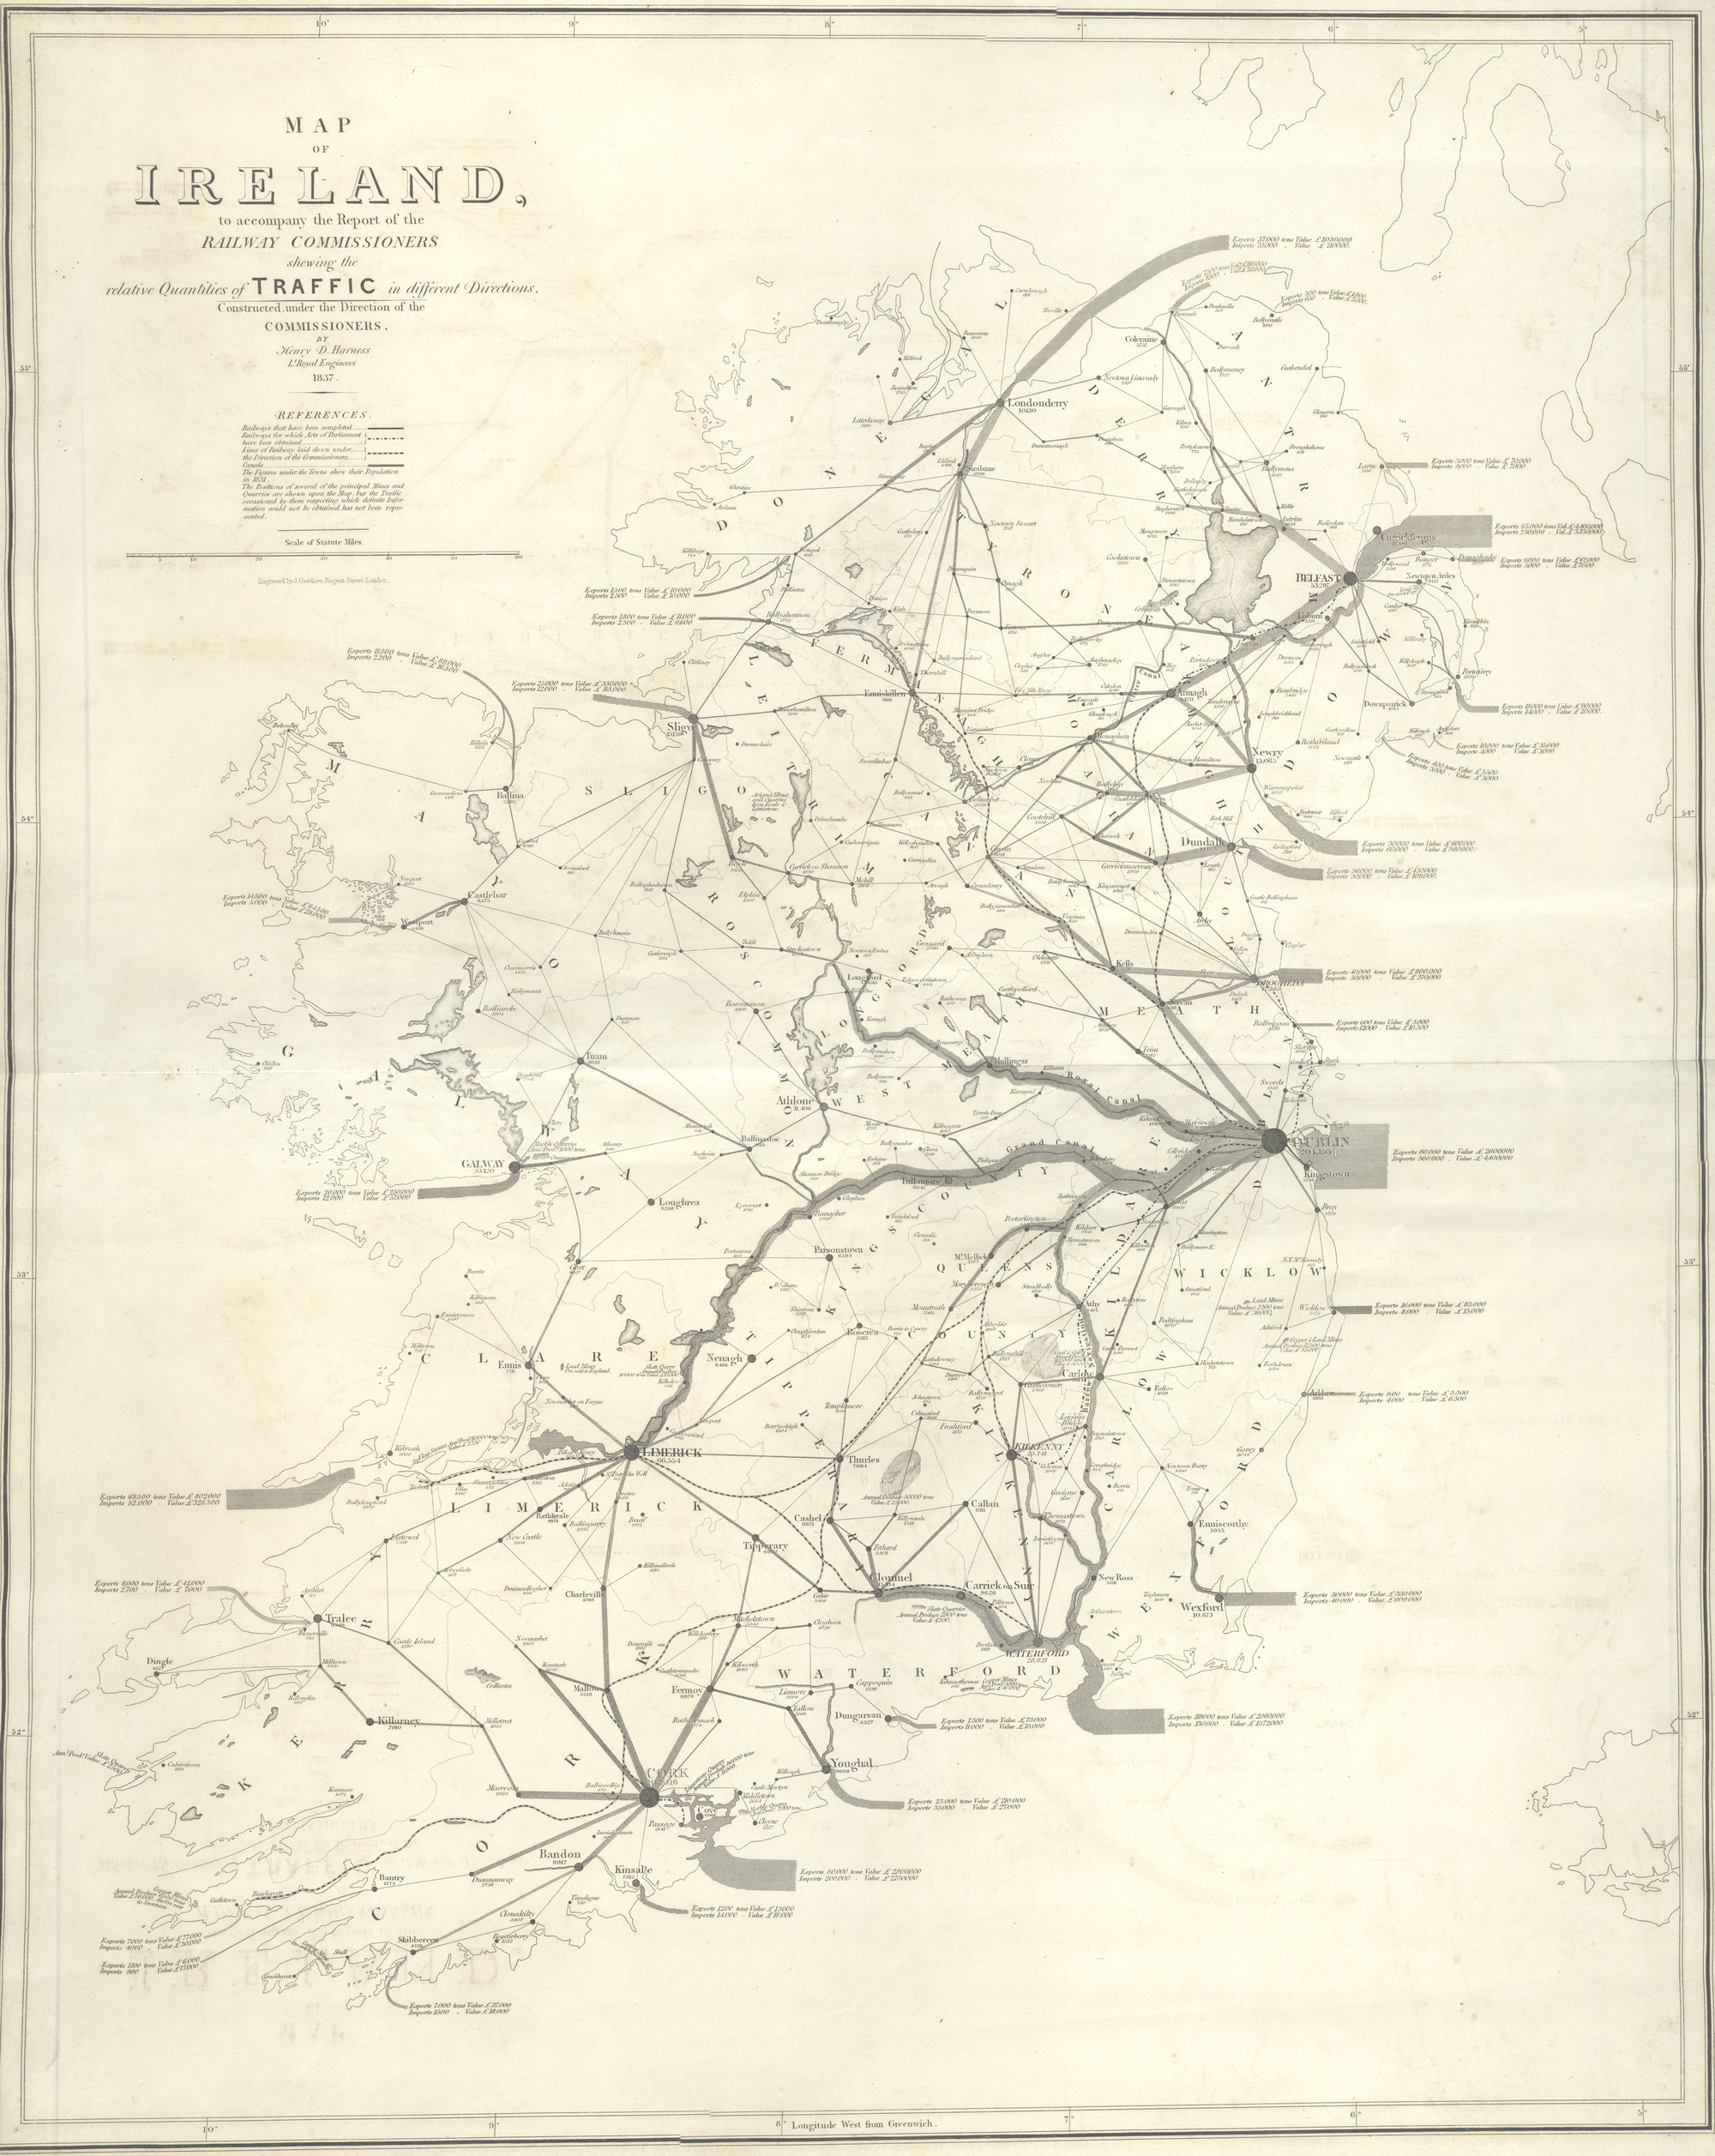
\includegraphics[width=\textwidth]{graphics/2-literature-review/14}
    \end{center}
    \caption{The flow of cargo traffic}
    \label{fig:figure2.14}
\end{figure}

\clearpage

Migrations of people can also be represented circularly. A popular visualization for this is a chord diagram where nodes are placed on
the outer part of the circle and connected among each other by arcs. The size of an arc, like the line in the flow map, is proportional to
the number of people or objects moving. Below we can see an example of a chord diagram taken from~\citep{baptista2018internal}. It shows the
migration flows in the Brazilian states between 2005 and 2010.

\begin{figure}[h]
    \begin{center}
        \includegraphics[width=0.7\textwidth]{graphics/2-literature-review/15}
    \end{center}
    \caption{A chord diagram of migration flow in Brazilian states (thousands)}
    \label{fig:figure2.15}
\end{figure}

Chord diagrams are often interactive because they allow a better visual aspect of the data. The static ones can seem tangled and hard to
understand if there are too many arcs. The interactive part usually allows the user to highlight only a selected arc, while others may change
the color to become less visible and neutral, and the selected one stands out for a better view.\footnote{You can see an example of an
interactive chord diagram on the website\\ \url{http://download.gsb.bund.de/BIB/global_flow/}}
Rees et al.~\citep{rees2020interaction} introduce more engaging interaction techniques for chord diagrams.

A very interesting data visualization of the migration of artists found in the Rijksmuseum database is the one by
Koeleman~\citep{koeleman2017visualizing}. In this interactive chart, it is possible to hover over the cities on the outer part of the circle
or a country in the inner part for the migrations related to it to lighten.\footnote{Chart can be found on the website
\url{http://visualizingvisions.com}} The red lines show the immigration patterns, while the blue ones show the emigration. We can see that most
of the artists are from the Netherlands (not surprising as the Rijksmuseum is in Amsterdam), but a more interesting discovery is that artists
from various nationalities moved to Italy, while the Italian ones only moved within the country.

\begin{figure}[h]
    \begin{center}
        \includegraphics[width=0.9\textwidth]{graphics/2-literature-review/16}
    \end{center}
    \caption{Migration of artists found in Rijksmuseum database}
    \label{fig:figure2.16}
\end{figure}

These visualizations show that the representation of the movement of people usually includes a big amount of data. It enables
searching for a pattern and understanding what happened in general, not focusing much on a single person as an object of observation. Besides, they
do not offer a lot of details about locations and their spatial relationships. Because we are interested in the life of an artist as an individual,
these types of data visualizations are not suitable for the implementation part. Even though exploring relationships with other artists as well
gives us more data to work with, it would still be ineffective to use them because they are only concerned with the migration part. Nevertheless,
characteristics can still be taken from these charts and implemented in our work. For example, the property of a width of a line we saw in
\Cref{fig:figure2.14} can be used in our space-time cube to represent some aspect of an artist's life, such as the number of artworks they have
created during a certain period or any other.

    \section{Data Visualization in Cultural Heritage}\label{sec:data-visualization-cultural-heritage}

In \Cref{sec:space-time-cube} we were presented with an example of the space-time cube concept in the cultural heritage domain.
Kraak~\citep{kraak2005timelines} showed the paintings collections using this interface with the time slider incorporated in it that allows the
user to choose a time period. There are other visualizations in the cultural heritage domain as well, so in this section, we will present and
discuss some of them.

Nowadays, galleries, libraries, archives, and museums (known as \emph{GLAM} institutions) are in charge of the preservation of cultural
heritage assets~\citep{windhager2018visualization}. When speaking about cultural heritage, we refer to tangible and intangible heritage,
see \Cref{fig:figure2.17}. Tangible includes all the physical assets like historical buildings, artifacts, sculptures, paintings, etc.
Intangible, on the other hand, includes traditions and skills, traditional knowledge, social ceremonies, and others.

\begin{figure}[hbt!]
    \begin{center}
        \includegraphics[width=\textwidth]{graphics/2-literature-review/17}
    \end{center}
    \caption{Examples of tangible and intangible assets~\citep{intavia}}
    \label{fig:figure2.17}
\end{figure}

Representing these assets visually by using some kind of interface is a challenging task. One of the main problems is the so-called “museum
fatigue”, where visitors are overwhelmed with the information they see, with computer screens making no exception~\citep{windhager2020many}.
These cultural heritage collections need to be visualized in a way where the most important dimensions of collected data, as seen in
\Cref{fig:figure2.18}, are presented so that the users can easily understand what they are seeing. This is mostly done by combining multiple
visualization types, such as maps with timelines, that allow users to form their own mental model~\citep{windhager2020many}.

\begin{figure}[hbt!]
    \begin{center}
        \includegraphics[width=\textwidth]{graphics/2-literature-review/18}
    \end{center}
    \caption{Digitization and visualization of cultural heritage collections~\citep{windhager2020many}}
    \label{fig:figure2.18}
\end{figure}

Now we will discuss a number of data visualization interfaces for cultural heritage collections before shifting our focus to the
visualization of artist biographies that belong to the intangible assets of cultural heritage.

\Cref{fig:figure2.19} shows the interactive timeline explorer by the Google Arts \& Culture~\citep{google} that displays artists in the
selected period. We can choose any artist from the ones shown and read everything related to them as well as explore their artworks.

\clearpage

\begin{figure}[hbt!]
    \begin{center}
        \includegraphics[width=0.95\textwidth]{graphics/2-literature-review/19}
    \end{center}
    \caption{Google Arts \& Culture interactive artists' timeline}
    \label{fig:figure2.19}
\end{figure}

Another similar example is The Museum of the World timeline, a collaboration between the British Museum and
the Google Arts and Culture Lab. Users can explore the museum’s collection by continent, discover connections between objects, filter
the area of interest and see additional information of each object as well~\citep{britishmuseumworld}.

\begin{figure}[hbt!]
    \begin{center}
        \includegraphics[width=0.95\textwidth]{graphics/2-literature-review/20}
    \end{center}
    \caption{The Museum of the World interactive timeline}
    \label{fig:figure2.20}
\end{figure}

Peripleo by Simon et al.~\citep{simon2016peripleo} is a prototype visualization tool for exploring heterogeneous data through the dimensions
of space and time. Users can search the geographic, temporal, and thematic composition of digital collections, furthermore filtering them to
analyze individual records. The paper provides a detailed description and examples of how to use the tool.

\begin{figure}[hbt!]
    \begin{center}
        \includegraphics[width=\textwidth]{graphics/2-literature-review/21}
    \end{center}
    \caption{Peripleo tool for exploring digital collections}
    \label{fig:figure2.21}
\end{figure}

Windhager et al.~\citep{windhager2018orchestrating} present the PolyCube interface for visualizing cultural heritage
data. It originates from the space-time cube representation and visualizes large data collections as a wide range of shapes or patterns.
The PolyCube framework incorporates several space-time cubes into a “coordinated multiple cubes” view~\citep{windhager2020many}.

\begin{figure}[hbt!]
    \begin{center}
        \includegraphics[width=\textwidth]{graphics/2-literature-review/21a}
    \end{center}
    \caption{PolyCube interface for visualizing cultural heritage data}
    \label{fig:figure2.21a}
\end{figure}

We will see an example of the PolyCube framework used to visualize the life and work of an artist in the next section.







    \section{Representing An Artist's Life}\label{sec:representing-artists-life}
If we think about how the artist’s life is presented to the public, we first speak of biography books and memoirs~\citep{isaacson2017leonardo,
    tomkins1999duchamp, herrera1983frida}, then museum exhibitions, articles and interviews, and others. Essentially, it is mostly a sort of
written form and in some cases includes visual aspects, like in exhibitions.

\begin{figure}[h!]
    \begin{center}
        \includegraphics[width=0.9\textwidth]{graphics/2-literature-review/22}
    \end{center}
    \caption{Biographical investigation of an individual and some usual types of visualizations~\citep{windhager2017synoptic}}
    \label{fig:figure2.22}
\end{figure}

The study of biographies has been a usual and important investigative perspective for centuries~\citep{windhager2017synoptic}. The paper also
states that biographical data is usually
\begin{enumerate}
    \item \emph{multidimensional} -- has spatial, relational, and categorical dimensions, and all of these are commonly.
    \item \emph{time-oriented} -- entities are linked to events or connected to timestamps.
\end{enumerate}

According to these properties of biographical data, we can see that the space-time cube is the suitable choice for our case. We have a
spatial dimension, as well as a relational dimension, and both of them are linked to the events in the artist’s life.

Mayr and Windhager~\citep{mayr2018once} list some common hybrid visualizations of spatial (brown) and temporal (orange) data dimensions,
including the space-time cube: a) multiple coordinated views, b) animation/slideshow, c) color-coded layer superimposition, d) layer
juxtaposition, e) space-time cube.

\begin{figure}[hbt!]
    \begin{center}
        \includegraphics[width=\textwidth]{graphics/2-literature-review/23}
    \end{center}
    \caption{Hybrid visualizations for spatial and temporal data dimensions}
    \label{fig:figure2.23}
\end{figure}

Usually, one-dimensional visualizations like maps and timelines only allow the analysis of single data dimensions and there is no space for
the examination of cross-dimensions. These hybrid visualizations can provide a visual comparison and combination of biographical patterns that
include the similarities and differences among several artists~\citep{windhager2017beyond}.

Capturing the essence of artists’ life furthermore depends on what we want to present. Is it related to their work only or do we include other
parameters as well - family connections, places they lived in, relations to other artists, or some others? Fitting such things as full knowledge of
an artist’s life into a few written pages or simple visualizations is a hard task to do. It is necessary to extract the most important aspects and
capture them in the best possible way. We will seek to do this in the implementation part of this thesis altering the previously seen space-time
cube. But before doing that, we need to present some already-seen visualizations associated with artists and their lives.

The first visualization is an anthology of ten painters’ lives by Giorgia Lupi and Michela Buttignol~\citep{lupi_buttignol}. They used
pictorial elements related to artists’ styles to present their lives visually. Each artist was presented with a timeline composed of the life
events and artworks using colors and shapes associated with their style. The example shown in \Cref{fig:figure2.24} is the life of Picasso.

\begin{figure}[hbt!]
    \begin{center}
        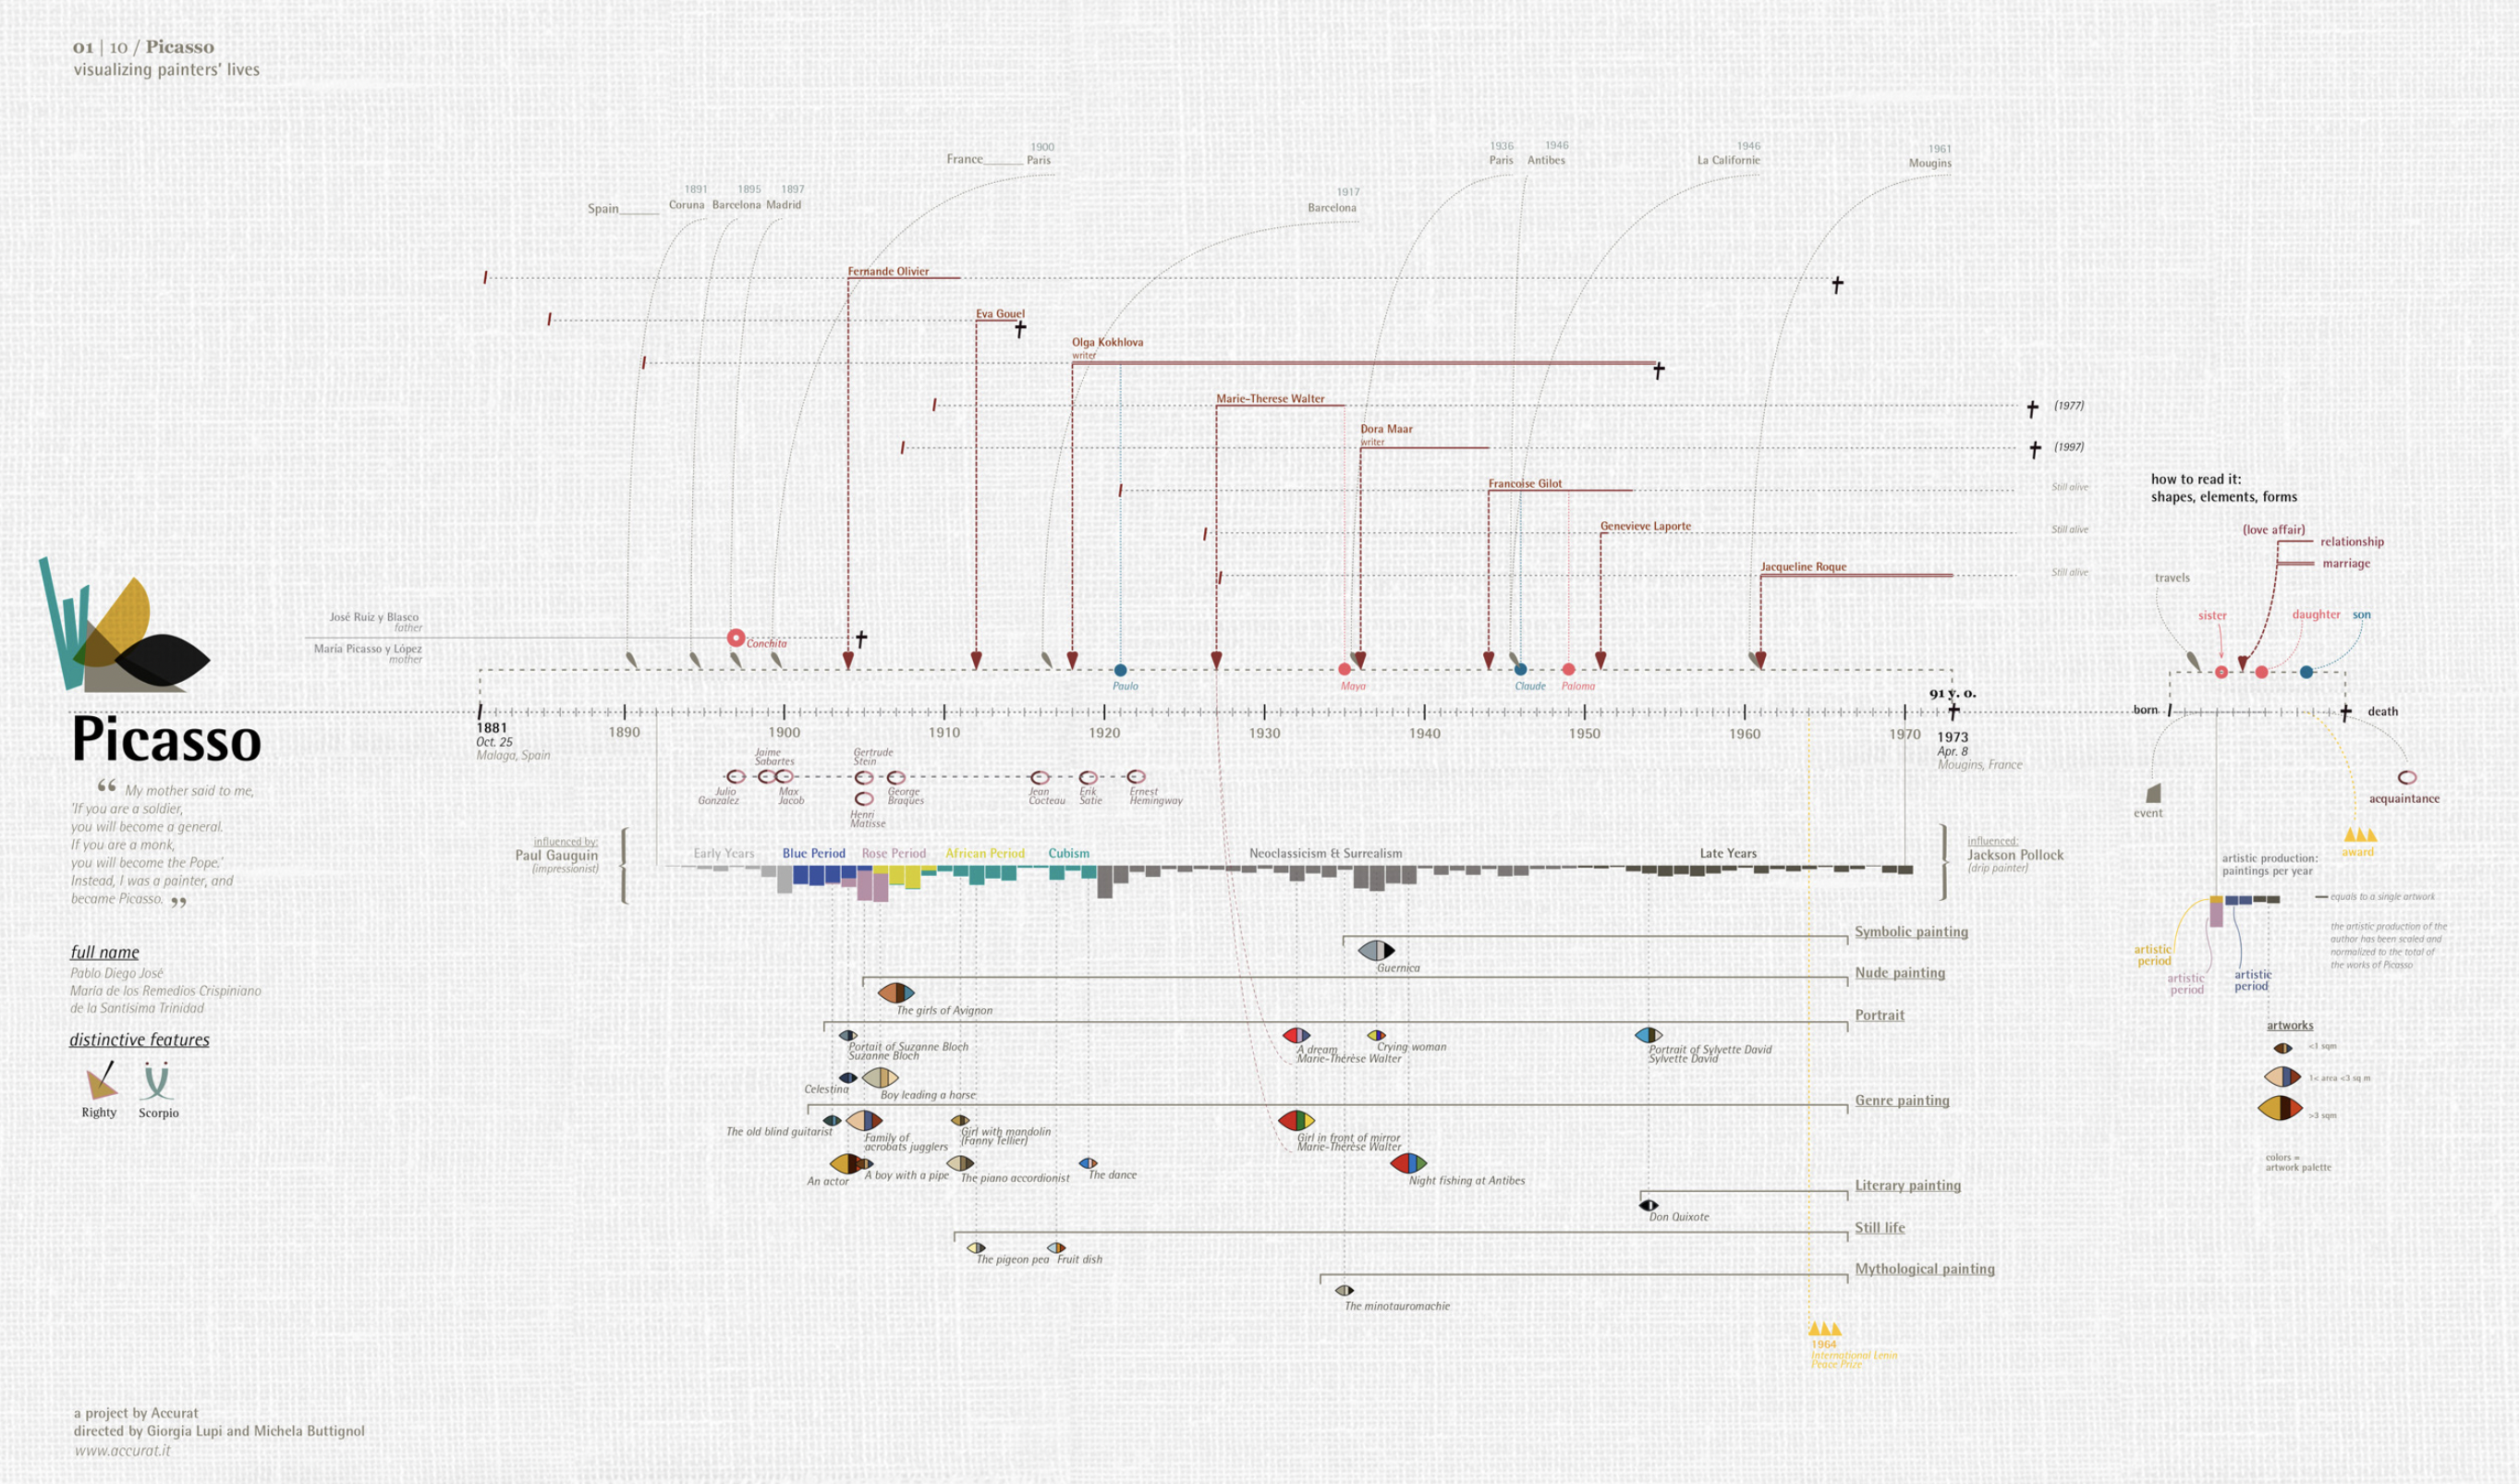
\includegraphics[width=1.3\textwidth, angle=90]{graphics/2-literature-review/24}
    \end{center}
    \caption{Pictorial representation of Picasso's life}
    \label{fig:figure2.24}
\end{figure}

\clearpage

We can see the timeline of the artist from his birthdate and birthplace to his death. Above the line are his love affair relationships with
some of them ending in marriage. This part also presents places he traveled to, his siblings, and his offspring, each colored
differently. Everything related to their personal life is shown in the upper part. The lower part is concerned with their artistic world. We
can spot the distinctive artistic periods and amount of works during that time, acquaintances, awards, and events. The most important part of
the visualization is the artworks where the painter’s masterpieces are presented in small shapes and colored according to the artwork’s
palette. All of them are also grouped according to the subject of the work. The pictogram’s size depends on the real painting size and is
divided into three categories: small, medium, and large. The visualization covers a lot of things related to the artist’s life, but everything
is explained thoroughly.

The second example is an interactive timeline of Andrew Wyeth’s life shown in the figure below~\citep{wyeth_2021}.

\begin{figure}[hbt!]
    \begin{center}
        \includegraphics[width=0.9\textwidth]{graphics/2-literature-review/25}
    \end{center}
    \caption{Andrew Wyeth’s life timeline}
    \label{fig:figure2.25}
\end{figure}

The left and right arrows allow the exploration of his life with the year indicators at the top. It is possible to skip to a certain year and
explore only that part. At the bottom, there is a search box for searching the timeline and showing only those events that contain a searched
term.\footnote{You can explore Andrew Wyeth's timeline at \url{https://andrewwyeth.com/timeline/}}

We have seen from the first two examples that they used the timeline to present the artist’s life. Drawing a straight line and arranging
life events, relationships, artworks, and everything else seems like an engaging way of capturing one’s life. The first example elevated the
conventional timeline and introduced innovative ways of showing all the details about the artist’s life. Although the visualization was
two-dimensional and not interactive, it was still an attractive solution. The second example was a typical timeline with photos and written
captions included. On the other hand, it had an interactive aspect which contributed to easier maneuvering and finding information of interest
faster.

\begin{figure}[hbt!]
    \begin{center}
        \includegraphics[width=\textwidth]{graphics/2-literature-review/26}
    \end{center}
    \caption{Inventing abstraction by MoMA}
    \label{fig:figure2.26}
\end{figure}

When speaking about the connections between artists, one example of it is presented in \Cref{fig:figure2.26}, the visualization by the
Museum of Modern Arts for the Inventing Abstraction exhibition~\citep{moma}. It is interactive and there is a possibility to click on any
artist in order to explore only their connections with others. Artists with their names in red are the ones with the most connections.

An example of the PolyCube framework (see \Cref{sec:data-visualization-cultural-heritage}) used in cultural heritage was the visualization
of the life and work of an amateur photographer Charles Weever Cushman~\citep{mayr2019visualizing}. Cushman’s work was presented using
geographic and categoric space-time cubes where each cube depicted a relevant pattern with the temporal development between 1938 and 1955.

\begin{figure}[hbt!]
    \centering
    \begin{subfigure}{.5\textwidth}
        \centering
        \includegraphics[width=0.9\linewidth]{graphics/2-literature-review/artist1}
    \end{subfigure}%
    \begin{subfigure}{.5\textwidth}
        \centering
        \includegraphics[width=\linewidth]{graphics/2-literature-review/artist2}
    \end{subfigure}
    \caption{Geographical (left) and categorical (right) space-time cube representations of Charles W. Cushman's life and  work}
    \label{fig:figure2.artist}
\end{figure}

The figure on the left shows the geographical pattern of the photographs where the earliest ones are colored in violet and the latest ones in
yellow. Scattered points mean the photographer was traveling extensively during that time. The figure on the right presents us with
categorical patterns based on the main photography genres. Each category was colored differently and dispersed among the timeline thus we can
examine the number of specific photograph genres taken every year. For example, in 1943 he took the least number of photos.

\clearpage

\begin{figure}[hbt!]
    \begin{center}
        \includegraphics[width=\textwidth]{graphics/2-literature-review/artist3}
    \end{center}
    \caption{Landscape genre filtered space-time cube representations of Charles W. Cushman's work}
    \label{fig:figure3.artist}
\end{figure}

The paper also shows the framework providing us with the possibility to filter the genre and present a “coordinated multiple cubes” view. In
the figure above, we can see the filtered landscape photographs and explore their spatio-temporal distribution closely.

    \clearpage
    \section{Strengths and Weaknesses of the Space-Time Cube}\label{sec:strengths-weaknesses-stc}
Before proceeding to the next chapter of this research, we need to address points of strength and weakness of the space-time cube as this
visualization technique will be used in the implementation part. We have seen multiple examples of space-time cube and their usage in
different domains. However, this visualization has its strengths and weaknesses like any other. We briefly mentioned some of them in
\Cref{sec:space-time-cube}, but we will present them in detail here and try to understand where improvements can be made.
Since we want to display various aspects related to an artist’s life, the objective of the visualization is to implement multidimensional data
while keeping the user’s cognitive load low.

Strengths of the space-time cube:
\begin{itemize}
    \item Proved to have unique strengths in showing the multidimensional data~\citep{windhager2016reframing}.
    This property is of great importance and the space-time cube permits to implement multiple dimensions without
    losing its efficiency.
    \item Integration of data into the spatio-temporal dimension is fair and balanced because the most effective variables are distributed
    equally to all sides~\citep{windhager2018orchestrating}.
    \item Can mediate between different temporal visualizations and translate from temporal to spatial perspectives
    while allowing seamless transitions. This makes it act as a translational hub or operational cognitive
    scaffold~\citep{windhager2018orchestrating}.
    \item Spatio-temporal patterns and clusters are identified more quickly and accurately with the space-time cube than with
    the 2D visualization~\citep{amini2014impact, kristensson2008evaluation}.
    \item Visual variables for 2D maps (size, shape, color, value, orientation, and texture) by Bertin~\citep{bertin1983semiology}
    can be applied to the space-time paths to represent quantity or quality differences of attribute information
    (color for distinguishing multiple space-time paths, path width for quantitative characteristics, and additional attachments to the
    space-time paths whose size, color, and shape represent quantity or quality difference of attributes)~\citep{song2021visualization}.
\end{itemize}

Weaknesses of the space-time cube:
\begin{itemize}
    \item Investigating and visualizing large collections in the space-time cube significantly increases the response time
    of the analysts~\citep{windhager2020many}.
    \item Visual clutters are formed when the number of space-time paths is larger than the capacity of the cube,
    therefore resulting in a small amount of efficient information that can be analyzed~\citep{song2021visualization}.
\end{itemize}

With this we have concluded the research on previous works. In the following chapter, the conceptual part of the thesis proposal which improves the
currently available implementations will be presented.


    \chapter{Background}\label{ch:background}
    In this chapter, we will talk about the conceptual development and implementation part of the thesis. As previously said, the space-time cube was chosen to present
artists' lives. Several technologies were used in order to implement this visualization, more about them was mentioned in \Cref{ch:background}.

The original concept of the space-time cube along with the examples we have seen was just the starting point of creating the visualization. It was
necessary to decide which parts of their lives to include in the cube. Also, it was necessary to decide which external events to integrate in it,
to make the visualization more meaningful. Additional information was included, like exhibitions artists attended, important stays in their life,
minor/major historical events that might have influenced artists' lives, connections between multiple artists, and others. These were combined
with the space-time path that represents the artists' movement during their life. Each of these parameters will be explained in detail and the
most important and interesting examples of the code will be mentioned.

\clearpage

Before presenting the implementation aspects of the representation of the space-time cube, we present parameters and features that were selected for the representation in the cube:
\begin{itemize}
    \item The first feature represents the space-time path of an artist's life. The path will show the activity during their life. This trajectory will include locations of their stays and the length of each stay. Some stays could be important for different reasons, because of this, they will be specially marked. The choice of this feature was rather obvious, because visualizing a movement path is the primary purpose of a space-time cube.
    \item The second feature is related to the artistic part of an artist's life. This includes the artworks they created during their life. During our literature review, we saw representations that only concentrated on the artist's work, but did not include information on the life. Adding this feature to the space-time path combines multiple different representations into a single one.
    \item The third important feature which will be included are connections between artists. We saw examples of representations that show connections and relations between people, so including this aspect of an artist's life in the same visualization allows us to explore multiple space-time paths and examine the potential connections and relations between artists.
    \item The fourth feature we decided to represent are the exhibitions. These play important part in the artists' lives because they reflect on events attended by multiple artists and can help art experts to determine faster which artists were connected by mutual exhibitions.
    \item The last feature that we decided to implement are records of historic events which might have influenced artists' lives. These will not be related to artists closely, but will be included in the visualization independently. By observing these events, users will be able to see if some of them influenced the artists' life paths, for example, caused them to move elsewhere.
\end{itemize}

Since this is a 3D visualization and the AR part is animated through a mobile device, only the screenshots of the visualization will be
included in this chapter.
    \clearpage
    \section{Angular}\label{sec:angular}
This section will give a basic introduction to Angular. The information was mostly taken from~\citep{angular} and~\citep{murray2018ng}
which can be consulted for further reference.

Angular is an open-source framework for web applications built on TypeScript. It was developed by Google in 2010 and the first version was
known as AngularJS. At the time of writing, the latest version is Angular 15 released in November 2022.

Angular, as a development platform, includes:
\begin{enumerate}
    \item A framework based on components for creating web applications.
    \item A number of libraries that include many features such as routing, forms management, client-server communication, and others.
    \item A set of developer tools for developing, building, testing, and updating the code.
\end{enumerate}

Components are the building blocks of Angular architecture. We use them as custom-made HTML tags that have specific functionalities linked to
them.

\begin{figure}[hbt!]
    \begin{center}
        \begin{lstlisting}[language=JavaScript,label={lst:angular-code-1},belowskip=-1 \baselineskip]
import { Component } from '@angular/core';

@Component({
    selector: 'app-home',
    templateUrl: './home.component.html',
    styleUrls: ['./home.component.css']
})

export class HomeComponent {
    // ...
}
        \end{lstlisting}
    \end{center}
    \caption{Example of an Angular component}
    \label{fig:figure4.1}
\end{figure}

The \texttt{import} statement specifies which modules to use to write the code. In this case, we are importing the
\texttt{Component} module. Next, we need to declare the component. \texttt{@Component} is called a decorator - which can be thought of as
metadata added to the code. The \texttt{selector} inside acts as a new tag to use in the HTML file of the component, so the tag will be
\texttt{<app-home>}. The \texttt{templateUrl} selector loads the template from the \texttt{home.component.html} file. The \texttt{styleUrls}
loads the CSS file associated to style the component. By default, the style will only apply to the given component and this approach Angular
uses is called \emph{style-encapsulation}.

After the component is created, it is necessary to load it. In order to do that, it is mandatory to add the component tag to the related template
file.

\begin{figure}[hbt!]
    \begin{center}
        \begin{lstlisting}[language=HTML,label={lst:angular-code-2},belowskip=-1 \baselineskip]
<div>
    <app-home></app-home>
</div>
        \end{lstlisting}
    \end{center}
    \caption{Loading Angular component in HTML file}
    \label{fig:figure4.2}
\end{figure}

This was a basic introduction to Angular with an example of creating and loading a simple component. The next section will give us
insight into the Three.js library, also used in the frontend.
    \section{Three.js}\label{sec:three.js}
This section presents the Three.js library. The mentioned information was taken from~\citep{dirksen2013learning}. Also, an
example~\citep{threejsdocs} will be presented of how to create a 3D cube.

Three.js is a JavaScript library and API (application programming interface) for creating 3D graphics in a web browser. It was released by
Ricardo Cabello in 2010 on GitHub. The library provides an easy-to-use JavaScript API around the WebGL features without having to learn WebGL
in depth since programming it directly is very complex and error-prone.

\clearpage

Three.js makes it easy to:
\begin{itemize}
    \item Build both simple and complex 3D geometries.
    \item Animate and move objects in a 3D scene.
    \item Add textures and materials to the objects.
    \item Use various light sources to illuminate the scene.
\end{itemize}

The main components for displaying anything with Three.js are the scene, camera, and renderer, which are used to render the scene with the
camera. Code example below shows how to create a simple 3D cube.

\begin{figure}[hbt!]
    \begin{center}
        \begin{lstlisting}[language=JavaScript,label={lst:threejs-code-1},belowskip=-1 \baselineskip]
const scene = new Scene();
const camera = new PerspectiveCamera( 75, window.innerWidth / window.innerHeight, 0.1, 1000 );
const renderer = new WebGLRenderer();
renderer.setSize( window.innerWidth, window.innerHeight );
        \end{lstlisting}
    \end{center}
    \caption{Main components in Three.js}
    \label{fig:figure4.3}
\end{figure}

The first line creates the scene, which is used to store objects. Then the camera object is created using the \texttt{PerspectiveCamera}.
Three.js has many additional cameras such as \texttt{ArrayCamera}, \texttt{CubeCamera}, \texttt{OrthographicCamera}, but the
\texttt{PerspectiveCamera} is the one that resembles how the human eye sees. There are multiple attributes the \texttt{PerspectiveCamera}
uses: field of view, aspect ratio, near, and far (respectively).

The renderer is defined next, and the library has additional renderers besides the \texttt{WebGLRenderer} for those who use older browsers or do not
have the support for WebGL. After creating the renderer instance, it is important to set the size at which to render the application. This is done by
using the \texttt{setSize()} function.

\clearpage

After the scene is created, it is necessary to create an object to add into the scene.

\begin{figure}[hbt!]
    \begin{center}
        \begin{lstlisting}[language=JavaScript,label={lst:threejs-code-2},belowskip=-1 \baselineskip]
const geometry = new BoxGeometry( 1, 1, 1 );
const material = new MeshBasicMaterial( { color: 0x00ff00 } );
const cube = new Mesh( geometry, material );
scene.add( cube );
camera.position.z = 5;
        \end{lstlisting}
    \end{center}
    \caption{Creating an object in Three.js}
    \label{fig:figure4.4}
\end{figure}

\texttt{BoxGeometry} creates a cube, and in addition to creating the cube, we need a material to color it. \texttt{MeshBasicMaterial} is one
of the available materials in the library, and it contains attributes such as: the color of the material, how reflective it is, whether it has
transparency, whether it emits light, how metallic it is, whether it should use a texture, etc. This allows us to easily define materials which mimic
their real world counterparts.

Lastly, everything is tied together by using a \texttt{Mesh} object to merge the geometry and corresponding material so
that it is possible to insert it into the scene. For this, the created object is added to the scene using \texttt{scene.add()}. To avoid the camera
and the cube being inside each other, the camera has to be moved out in a proper position.

After the scene and the object within it are specified, the last thing to do is to render the scene using the function \texttt{animate()}.

\begin{figure}[hbt!]
    \begin{center}
        \begin{lstlisting}[language=JavaScript,label={lst:threejs-code-3},belowskip=-1 \baselineskip]
function animate() {
    requestAnimationFrame( animate );
    renderer.render( scene, camera );
}
        \end{lstlisting}
    \end{center}
    \caption{Rendering the scene in Three.js}
    \label{fig:figure4.5}
\end{figure}

\clearpage

    \section{WebXR}\label{sec:webxr}
This section presents WebXR. The information was mostly taken from~\citep{webapismdnwebxr}.

WebXR is an API for web content that uses augmented (AR) or virtual reality (VR). It was developed by Mozilla in 2014 under the name WebVR.
Later in 2018, with the addition of AR, it was merged into WebXR. Both AR and VR paradigms belong to the mixed reality (MR) or cross
reality (XR), hence the name. However, WebXR does not support rendering of objects. This is entirely up to the developer, that they can use the previously mentioned WebGL API\@.

WebXR and its features are not supported on all browsers and versions,\footnote{Information on which browsers support
WebXR and corresponding features can be found at \\ \url{https://developer.mozilla.org/en-US/docs/Web/API/WebXR_Device_API} and
\url{https://immersiveweb.dev}} so it is still in active development at the time of writing. This may present a limitation for some projects
because developers have to take into consideration the device type, the environment in which it will be used, etc.

As we already said, WebXR supports both augmented reality and virtual reality. Which one we want to use depends on the type of experience
we want to create for the user. Each paradigm requires a different approach and sometimes also a specific device for visualizing the project.

VR and AR paradigms are mapped to:
\begin{enumerate}
    \item Virtual reality -- the entire image we see is digitally created by the application. There are two VR modes available: \emph{inline} and
    \emph{immersive-vr}. The first one is rendered within the web browser and does not require special hardware device to display. The latter
    requires a headset to render the scene which can be seen by the user’s eyes.
    \item Augmented reality -- this mode renders the image in the real-world environment around us. Since this is always an immersive
    experience, we only have one mode -- \emph{immersive-ar}. Types of devices that can be used to explore AR are phones/tablets and transparent
    glasses.
\end{enumerate}

In the implementation part, in order to visualize the cube in AR mode, we used the latest Chrome version on an Android device and the
XRViewer application for an iPhone device.

For further reference and a deeper understanding of how to create an application in AR/VR, please refer to~\citep{baruah2021ar}.

    \section{The Spring Framework}\label{sec:spring-framework}
The Spring Framework is used for the backend of the implementation. Information on the
framework was mostly taken from~\citep{springframework, johnson2004spring}, as well as~\citep{walls2022spring}. They can be looked at for
further reference. Code examples are taken from our project.

Spring is an open-source framework for building Java applications. It also supports the Kotlin programming language, which has been used for our
implementation. The first release was in 2002 and the latest version, at the time of writing, is Spring Framework 6.0. It is extremely
lightweight (both in size and overhead), being distributed in a file of just over 1 MB\@.

The framework is split into many modules that are grouped into several layers. We do not have to use each one of the modules but choose them
according to the application's architecture and requirements. All modules are built on the top of the core container which includes the
configuration model and a dependency injection mechanism.

\Cref{fig:figure4.6} shows all the Spring layers and modules, and what each of them does is briefly explained below.

The Spring Framework module layers include:

\begin{enumerate}
    \item Core Container -- includes four modules, with Beans and Core providing the integral functionality of the framework -
            IoC (\emph{Inversion of Control}) and DI (\emph{Dependency Injection}).
    \item Data Access/Integration -- includes five modules used for data handling and integration. One of them is ORM (\emph{Object Relational
            Mapping}) which provides several object-relational mapping APIs, including JPA (\emph{Java Persistence API}), which we use in our
            implementation.
    \item Web -- this layer includes four modules. One of them, Web, is used in our implementation and it provides web-oriented integration
            features.
    \item AOP, Aspects, and Instrumentation -- AOP module provides aspect-oriented programming implementation, while the Aspects module
            supports integration with AspectJ. The instrumentation module provides class instrumentation support which is used in some
            application servers.
    \item Test -- this module, as the name states, supports testing of the components with JUnit or TestNG\@.
\end{enumerate}

\begin{figure}[hbt!]
    \begin{center}
        \includegraphics[width=0.9\textwidth]{graphics/4-background/1}
    \end{center}
    \caption{Spring Framework Layers and Modules~\citep{introtospringframework}}
    \label{fig:figure4.6}
\end{figure}

Since we mentioned that we use some of the modules in our implementation, namely ORM and Web, we will now explain them more in detail, as well
as the concept of dependency injection and inversion of control.

\subsection{Dependency Injection}\label{subsec:dependency-injection}

We spoke about inversion of control and dependency injection mechanisms, but what do they actually do? Inversion of control is at the core of
Spring Framework. Almost every application nowadays consists of many classes and they need to collaborate with each other. In
general, every object has to obtain its own reference to the object it is working with (its dependencies), which is not really efficient.
This is why, by applying inversion of control, objects are given their dependencies at the time they are created by an external entity. This
means that dependencies are \emph{injected} into objects. By using IoC, we invert the responsibility of how the object obtains references to
the objects it is collaborating with.

Now, an example of how to declare a CityController class in Spring whose constructor contains two private parameters will be shown.

\begin{figure}[hbt!]
    \begin{center}
        \begin{lstlisting}[language=Kotlin,label={lst:spring-code-1},belowskip=-1 \baselineskip]
@RestController
class CityController(
        private val cityRepository: CityRepository,
        private val cityMapService: CityMapService,
)
        \end{lstlisting}
    \end{center}
    \caption{Declaring a class in Spring Framework}
    \label{fig:figure4.7}
\end{figure}

When a class is declared, the constructor is simply given all the objects needed in that class. Spring gives those objects during the
creation of an instance of a class, or even the implementation if it is an interface. These objects are called \emph{beans}. A bean can take
other beans in the constructor, or can itself be given to those who require it. Beans are declared with the help of annotations such as
\texttt{@Component}, \texttt{@Service}, \texttt{@Repository}, \texttt{@RestController}, etc.

\subsection{Object Relational Mapping (ORM)}\label{subsec:object-relational-mapping}

With the use of ORM, the main goal is to avoid writing SQL statements manually. In order to do this, first an entity is defined using the
\texttt{@Entity} annotation. Below is our example of a \texttt{City} entity. This entity represents a single table row in the
database. It contains all the columns that are found in that row, such as \texttt{id}, \texttt{name}, \texttt{x}, and \texttt{y}.

The first column (\texttt{id}) is annotated with \texttt{@Id} and it represents the primary key. Using \texttt{@GeneratedValue} annotation, Spring
generates the primary key value by itself and increments it automatically in our case. The rest of the columns in this entity are annotated
with \texttt{@Column}. There are other annotations for the columns like \texttt{@OneToMany}, \texttt{@ManyToOne},\texttt{@ManyToMany}, etc.
Based on this entity, Spring will automatically generate the corresponding table.

This is an advantage of Spring since the manually written SQL was not used to create the table, thus if the database needs some changes later,
the same code will work with MySQL, Postgres, H2, and others.

\begin{figure}[hbt!]
    \begin{center}
        \begin{lstlisting}[language=Kotlin,label={lst:spring-code-2},belowskip=-1 \baselineskip]
@Entity
data class City(
        @Id
        @GeneratedValue(strategy = GenerationType.IDENTITY)
        val id: Long? = null,
        @Column
        val name: String,
        @Column
        val x: Double,
        @Column
        val y: Double,
)
        \end{lstlisting}
    \end{center}
    \caption{Example of a Spring Framework entity}
    \label{fig:figure4.8}
\end{figure}

The data in the database is accessed over the repositories. These repositories are just interfaces, not classes that need to be implemented, and
Spring creates the instance of an interface by itself. Interfaces in our project implement \texttt{JpaRepository} which already has some predefined
methods such as \texttt{findAll()} for returning all instances of the type, \texttt{deleteById()} for deleting entity with the given ID,
\texttt{save()} for saving a given entity, etc. If more complex queries are needed, the methods can be added to the interface and Spring will
automatically create the query based on the method name, its parameter types, and the return type.\footnote{More on supported query method
predicate keywords, modifiers and return types at \\ \url{https://docs.spring.io/spring-data/jpa/docs/current/reference/html/}} Examples of these
methods can be seen in the code below: \texttt{findByName()} takes the city name and returns the whole \texttt{City} object if
there is one by that name, and \texttt{deleteByName()} method. If something beyond the queries that Spring can generate on its own is needed, the
regular full SQL query can be written as well.

\begin{figure}[hbt!]
    \begin{center}
        \begin{lstlisting}[language=Kotlin,label={lst:spring-code-3},belowskip=-1 \baselineskip]
@Repository
interface CityRepository : JpaRepository<City, Long> {
    fun findByName(name: String): City?
    fun deleteByName(name: String)
}
        \end{lstlisting}
    \end{center}
    \caption{Example of a Spring Framework repository}
    \label{fig:figure4.9}
\end{figure}

\subsection{Web}\label{subsec:web}

Our project's API is considered \emph{REST-like}, not completely the same as the actual REST architecture according to their specification, as it
does not comply with every detail of it. As we have already seen, the controller is annotated with \texttt{@RestController} so Spring knows it is a
bean. \texttt{@RequestMapping} gives the route name for all the methods that belong to that controller. Spring gives us all objects we need in
the constructor because of the already-mentioned dependency injection. Other routes are defined with the help of annotations like
\texttt{@DeleteMapping} in the \texttt{delete()} method. \texttt{POST}, \texttt{GET} and \texttt{DELETE} are set as methods, and data can be
obtained in different ways. The data the method returns is by default serialized into JSON format, but other return formats can be configured
as well.

\clearpage

This is an example of a controller from our project.

\begin{figure}[hbt!]
    \begin{center}
        \begin{lstlisting}[language=Kotlin,label={lst:spring-code-4},belowskip=-1 \baselineskip]
@RestController
@RequestMapping("api/v1/city")
class CityController(
        private val cityRepository: CityRepository,
) {

    @PostMapping
    fun post(@RequestBody city: City) {
        cityRepository.save(city)
    }

    @GetMapping
    fun get(): List<City> {
        return cityRepository.findAll()
    }

    @Transactional
    @DeleteMapping("/{name}")
    fun delete(@PathVariable name: String) {
        cityRepository.deleteByName(name)
    }
}
        \end{lstlisting}
    \end{center}
    \caption{Example of a Spring Framework controller}
    \label{fig:figure4.10}
\end{figure}



    \chapter{Concept and Implementation}\label{ch:implementation}
    In this chapter, we will talk about the conceptual development and implementation part of the thesis. As previously said, the space-time cube was chosen to present
artists' lives. Several technologies were used in order to implement this visualization, more about them was mentioned in \Cref{ch:background}.

The original concept of the space-time cube along with the examples we have seen was just the starting point of creating the visualization. It was
necessary to decide which parts of their lives to include in the cube. Also, it was necessary to decide which external events to integrate in it,
to make the visualization more meaningful. Additional information was included, like exhibitions artists attended, important stays in their life,
minor/major historical events that might have influenced artists' lives, connections between multiple artists, and others. These were combined
with the space-time path that represents the artists' movement during their life. Each of these parameters will be explained in detail and the
most important and interesting examples of the code will be mentioned.

\clearpage

Before presenting the implementation aspects of the representation of the space-time cube, we present parameters and features that were selected for the representation in the cube:
\begin{itemize}
    \item The first feature represents the space-time path of an artist's life. The path will show the activity during their life. This trajectory will include locations of their stays and the length of each stay. Some stays could be important for different reasons, because of this, they will be specially marked. The choice of this feature was rather obvious, because visualizing a movement path is the primary purpose of a space-time cube.
    \item The second feature is related to the artistic part of an artist's life. This includes the artworks they created during their life. During our literature review, we saw representations that only concentrated on the artist's work, but did not include information on the life. Adding this feature to the space-time path combines multiple different representations into a single one.
    \item The third important feature which will be included are connections between artists. We saw examples of representations that show connections and relations between people, so including this aspect of an artist's life in the same visualization allows us to explore multiple space-time paths and examine the potential connections and relations between artists.
    \item The fourth feature we decided to represent are the exhibitions. These play important part in the artists' lives because they reflect on events attended by multiple artists and can help art experts to determine faster which artists were connected by mutual exhibitions.
    \item The last feature that we decided to implement are records of historic events which might have influenced artists' lives. These will not be related to artists closely, but will be included in the visualization independently. By observing these events, users will be able to see if some of them influenced the artists' life paths, for example, caused them to move elsewhere.
\end{itemize}

Since this is a 3D visualization and the AR part is animated through a mobile device, only the screenshots of the visualization will be
included in this chapter.
    \section{General Overview}\label{sec:general-overview}
Before every part of our implementation is explained in detail, some general information about the visualization will be mentioned. As it will be detailled in \Cref{ch:background},
a web application for visualizing the space-time cube was implemented. It consists of frontend and backend parts. For the frontend part, Angular,
Three.js, and WebXR technologies were used, and for the backend part, Spring Framework.

\subsection{Backend}\label{subsec:backend}
The task of the backend was to manage the data -- save the information the user enters and provide the appropriate ones during the creation of the
cube. Since the cube is a spatio-temporal representation, for the spatial part some sort of a map was needed. The users enter the required cities on the
entire map by themselves, and the backend part manages the selection of the right portion of the map based on the provided cities for the chosen artists.
Including the whole map of the world in the cube would not be practical as only the part the artists lived in is important. More about this
concept will be discussed later in \Cref{subsec:map-cropping}.

The data types included in our database, not counting the helper tables, are \texttt{Artist}, \texttt{City}, \texttt{Residence}, \texttt{Exhibition}, and
\texttt{HistoricEvent}. \texttt{Artist} contains the name, the surname, and the list of locations artists lived in during their life. \texttt{City}
contains the city name and the city's x and y coordinates on the map. \texttt{Residence} contains the city name, the start and end date, the number of
artworks the artist created during their stay, and a label to describe if the stay was important and why. \texttt{Exhibition} contains the title of the
exhibition, the city where it was held, its start and end date, and the list of artists who attended it. \texttt{HistoricEvent} entity looks very similar,
but instead of the list of the artists, it contains the list of the cities where the event took place. More about the structure of the backend is
available in \Cref{sec:specifics-backend-implementation}.

\clearpage

\subsection{Frontend}\label{subsec:frontend}
The frontend is the web application which the user sees and interacts with. The application gives access to several functionalities such as:

\begin{itemize}
    \item managing the cities on the map,
    \item managing the list of artists,
    \item managing the exhibitions artists attended,
    \item managing the historical events that may have influenced artists' work.
\end{itemize}

For the presentation of the cube, the user has two options:

\begin{itemize}
    \item running the representation in a desktop web browser,
    \item running the representation in an AR viewer for mobile devices.
\end{itemize}

Everything on the frontend part is managed by the user. None of the data is taken via external sources, so the user has full control of it.

    \section{Homepage}\label{sec:homepage}
A short description of each of the functionalities is available for the user on the homepage of the application, seen in \Cref{fig:figure3.1}.
Nevertheless, they will be explained here as well.

The first step for creating the representation is to enter the cities the artist lived in, using a map. The map already shows all the available cities
from the previously entered artists. After entering the cities, the artist's information is entered. Finally, external events like exhibitions and historic events
can be entered, so that they can be represented in the cube as well.

Each functionality will be described in detail in the following sections.

\clearpage

\begin{figure}[hbt!]
    \begin{center}
        \includegraphics[width=\textwidth]{graphics/3-implementation/1}
    \end{center}
    \caption{Homepage view of the web application}
    \label{fig:figure3.1}
\end{figure}
    \section{Managing Cities}\label{sec:managing-cities}
The first functionality available to the user is to manage cities on the map. Several maps are available for selection, which are later, during the
visualization of the cube, cropped to the portion containing only cities relevant to the selected artists. This feature is important as it
dynamically changes the map to our needs, so the whole map with irrelevant locations is not included in the cube. Cities are added with a click on
the map using a small zoom-in lens, and their names and positions can be edited or deleted as well. During the addition of cities, their names are
entered in a modal dialog.

More information about how the map is cropped according to the artists’ residences, and the related parts of the project code, can be found in
\Cref{subsec:map-cropping}.

\begin{figure}[hbt!]
    \begin{center}
        \includegraphics[width=\textwidth]{graphics/3-implementation/2}
    \end{center}
    \caption{Manage cities functionality page}
    \label{fig:figure3.2}
\end{figure}

\clearpage
    \section{Managing Artists}\label{sec:managing-artists}
The \emph{Manage artists} page lists all the artists whose information has already been entered. Each artist's entry contains short information on
the number of inserted locations the artist has lived in during a period of time. These entries can be edited or deleted if necessary.

\begin{figure}[hbt!]
    \begin{center}
        \includegraphics[width=\textwidth]{graphics/3-implementation/3}
    \end{center}
    \caption{Manage artists functionality page}
    \label{fig:figure3.3}
\end{figure}

The main functionality on this page is the addition of new artists. Selecting this option gives the user a dialog for entering all the information
related to the artists' lives, such as their name, surname, and details about the cities they lived in. Each artist’s residence includes the date
from and date until which they lived there, information related to artworks during this stay, and an option to mark the stay as important or not.
If this option is selected, a textbox appears and the user can enter a short description of why the stay was important.

\Cref{sec:impl-stc} will show how this information is presented in the cube.

\begin{figure}[hbt!]
    \begin{center}
        \includegraphics[width=\textwidth]{graphics/3-implementation/4}
    \end{center}
    \caption{Adding a new artist dialog}
    \label{fig:figure3.4}
\end{figure}

\clearpage
    \section{Managing Exhibitions}\label{sec:managing-exhibitions}
The \emph{Manage exhibitions} page is similar to the \emph{Manage artists} page. Here, the list of exhibitions is presented. Every exhibition can
be edited or deleted, similar to the artist list. Each entry shows where and when the exhibition took place, together with the list of artists
that attended the exhibition.

\begin{figure}[hbt!]
    \begin{center}
        \includegraphics[width=\textwidth]{graphics/3-implementation/5}
    \end{center}
    \caption{Manage exhibitions functionality page}
    \label{fig:figure3.5}
\end{figure}

The main functionality is adding new exhibitions. A dialog is shown with several fields for entering information about the exhibition: the title of
the exhibition, the city it took place in, the start and end date. After entering this information, the user is presented with the list of artists
that lived in the chosen city during the selected time period. In this way, the list of all artists is not given, preventing the user from
selecting any artist that may have not been present at that place during that time. This constraint assures that the list of possible options of
artists that may have attended the exhibition is always accurate.

\clearpage

\begin{figure}[ht!]
    \begin{center}
        \includegraphics[width=0.7\textwidth]{graphics/3-implementation/6}
    \end{center}
    \caption{Adding a new exhibition dialog}
    \label{fig:figure3.6}
\end{figure}
    \section{Managing Historic Events}\label{sec:managing-historic-events}
The \emph{Manage historic events} page's functionality is to give the user the possibility to enter information on historic events. The list of
events is presented on the main page. Each event can be edited or deleted as well. Historic event entries show where and when the event took place. This
functionality is related to entering information on historic events that may have influenced artists' lives or work. They are not directly
associated to artists, but presenting them in the cube might give us an insight on what events possibly impacted artists' lives. Some of them might
have triggered a migration of artists to other cities or caused a change in their artistic works. Exploring the relationship between these
historic events and artists' lives gives experts additional interest in why changes happened in the first place.

This concludes the first part of the visualization -- entering data about the artist's life. The next step is running the
visualization. Firstly, visualizing the cube in the browser will be presented, and then the AR version of the visualization.

\clearpage
    \section{Space-Time Cube}\label{sec:impl-stc}
After the insertion of the data, the cube representation is run in the browser/viewer. Before the cube is presented, the list of the artists will
pop up, and the user needs to select those artists that they wish to visualize. This can either be a single artist, if only one life is to be
explored, or multiple artists if the connections between them are deemed important.

\begin{figure}[hbt!]
    \begin{center}
        \includegraphics[width=\textwidth]{graphics/3-implementation/9}
    \end{center}
    \caption{Selection of artists for the visualization of the space-time cube}
    \label{fig:figure3.9}
\end{figure}

\subsection{3D Web Browser Version}\label{subsec:3d-version}
The first presentation of the space-time cube is the 3D web browser version. The cube uses two dimensions to
represent the spatial dimension, and the third one to represent time. On the bottom of the cube, the map is shown. It includes all the cities
that the artists lived in, represented with small dots on the map. The main element in the cube is the space-time path. It shows the artists'
lives trajectories. Vertical lines represent the stay in each city and the length of them depends on how long the stay
was. If the stay was marked as important, it is colored and labeled differently. The user can click
on these labels and read information about why the stay was important. Marking the stay as important and describing it was mentioned in
\Cref{sec:managing-artists}. The third dimension contains a timeline with year labels. These can be modified to show the whole date as well.

The toolbar gives us multiple filtering options related to a number of variables, among which are: seeing the artists' number of artworks,
connections to other artists, exhibitions and historic events. Each of the options is presented differently in the cube, using distinct labels,
and their meaning is explained in the toolbar. On the top of the page is a button which gives the user the possibility to switch to 2D mode. More
about this will be explained in \Cref{subsec:time-flattened-version}.

\begin{figure}[hbt!]
    \begin{center}
        \includegraphics[width=0.9\textwidth]{graphics/3-implementation/10}
    \end{center}
    \caption{Space-time cube visualization in a web browser}
    \label{fig:figure3.10}
\end{figure}

\clearpage

\subsection{Time-Flattened Browser Version}\label{subsec:time-flattened-version}
The other version of the visualization that can be presented in the browser is the time-flattened cube which shows only a two-dimensional map. This
operation of time flattening has been mentioned in \Cref{sec:space-time-cube} and seen in \Cref{fig:figure2.9}. The reason behind introducing
this option is to concentrate only on the spatial trajectory of the artist's life without giving full details about time (the trajectory depends on
time, but the temporal intervals are not explicit anymore). This way, artists' trajectories can be observed with a main focus on spatial
movement and some other aspects related to it.

\begin{figure}[hbt!]
    \begin{center}
        \includegraphics[width=0.8\textwidth]{graphics/3-implementation/11}
    \end{center}
    \caption{Time-flattened space-time cube}
    \label{fig:figure3.11}
\end{figure}

\clearpage

\subsection{General Technical Features of the Space-Time Cube}\label{subsec:technical-specifics-stc}
Before moving to the AR presentation, we discuss some details related to the implementation of the space-time cube.

\subsubsection{Generating the Timeline}

For generating the timeline for our representation of the cube, at least two years are needed to be used as the initial and end year. The cube
takes the list of selected artists. It then looks at where and when the artists lived, to determine the initial and the final years any of the
selected artis lived in. In the coordinate system of Three.js, the initial year should be mapped to the $y=-0.5$ coordinate, since this is the
lowest point of the cube. Similarly, the final year should be mapped to the $y=0.5$ coordinate. This concept is illustrated in the figure below.

\vspace{0.5cm}

\begin{figure}[hbt!]
    \begin{center}
        \begin{tikzpicture}
            \draw[-] (-3.0,0) -- (3.0,0) ; %edit here for the axis
            \draw[gray,dashed,->] (-3, -0.7) -- (-3, -1.7);
            \draw[gray,dashed,->] (3, -0.7) -- (3, -1.7);

            \draw[shift={(-3,0)},color=black] (0pt,3pt) -- (0pt,-3pt);
            \draw[shift={(3,0)},color=black] (0pt,3pt) -- (0pt,-3pt);

            \draw[shift={(-3,0)},color=black] (0pt,0pt) -- (0pt,-3pt) node[below]
                {$1980$};
            \draw[shift={(3,0)},color=black] (0pt,0pt) -- (0pt,-3pt) node[below]
                {$2000$};

            \draw[-] (-3.0,-2) -- (3.0,-2) ; %edit here for the axis
            \draw[shift={(-3,-2)},color=black] (0pt,3pt) -- (0pt,-3pt);
            \draw[shift={(3,-2)},color=black] (0pt,3pt) -- (0pt,-3pt);

            \draw[shift={(-3,-2)},color=black] (0pt,0pt) -- (0pt,-3pt) node[below]
                {$-0.5$};
            \draw[shift={(3,-2)},color=black] (0pt,0pt) -- (0pt,-3pt) node[below]
                {$0.5$};
        \end{tikzpicture}
    \end{center}
    \caption{Mapping of years in the space-time cube}
    \label{fig:figure3.12}
\end{figure}

Naturally, we can achieve the desired result using a linear mapping. Let $m$ be the minimum year and $M$ be the maximum year. Then, the following
function can be used to map any year $y$ to the range $[-0.5,\ 0.5]$:

\begin{align*}
    f(y) = \frac{y - m}{M - m} - \frac 12
\end{align*}

Additionally, mapping the earliest and the latest years to the edges of the cube is not visually pleasing. Because of this, a small padding of a
few years is added to both minimum and the maximum year before defining the function $f$ so that the real minimum and maximum year values appear a
bit further away from the edge.

\clearpage

\subsubsection{Placing the Cities}

As we mentioned in \Cref{sec:managing-cities}, the whole map is not presented in the cube, only the portion which contains cities that the
selected artists lived in. However, when the cube receives the information about the cities in which the artists lived from the backend,
the coordinates of those cities are relative to the positions on the original map. These coordinates need to be adjusted to the cropped portion of
the map to retain the correct positions. In order to achieve this, the backend sends the coordinates of the upper-left and the bottom-right corners
of the cropped map relative to the original map. Based on this, we can create a mapping algorithm that maps the coordinates of the original map to
the coordinates of the cropped map.

The figure below presents the mapping and is followed by a detailed explanation.

\begin{figure}[hbt!]
    \begin{center}
        \begin{tikzpicture}
            \draw[-] (-5, -5) -- (-5, 5);
            \draw[-] (-5, 5) -- (5, 5);
            \draw[-] (5, -5) -- (5, 5);
            \draw[-] (-5, -5) -- (5, -5);
            %
            \draw[dashed] (-3, -3) -- (-3, 3);
            \draw[dashed] (-3, 3) -- (3, 3);
            \draw[dashed] (3, -3) -- (3, 3);
            \draw[dashed] (-3, -3) -- (3, -3);
            %
            \draw[dotted] (-1, 3) -- (-1, 0);
            \draw[dotted] (-3, 0) -- (-1, 0);
            %
            \node[] at (-5, 5.2) {\footnotesize $(0.0,0.0)$};
            \node[] at (5, -5.2) {\footnotesize $(1.0,1.0)$};
            %
            \node[] at (-3, 3.2) {\footnotesize $(0.2,0.2) \mapsto (0.0, 0.0)$};
            \node[] at (3, -3.2) {\footnotesize $(0.8,0.8) \mapsto (1.0, 1.0)$};
            \node[] at (-1, -0.2) {\footnotesize $(0.4,0.5) \mapsto (0.\overline 3,0.5)$};
            %
            \node at (-1,0) [circle,fill,inner sep=1.5pt]{};
        \end{tikzpicture}
    \end{center}
    \caption{Mapping the coordinates of the cities}
    \label{fig:figure3.13}
\end{figure}

As seen in \Cref{fig:figure3.13}, the upper-left corner of the original map which is presented as the outer square, has the coordinates
$(0.0,\ 0.0)$, whereas the lower-right one has the coordinates $(1.0,\ 1.0)$. If we want to map the coordinates $(0.4,\ 0.5)$ from the original
map to the cropped one, this can be again achieved by linear mapping. This mapping needs to map the upper-left and the lower-right corner of the
new map to the coordinates $(0.0,\ 0.0)$ and $(1.0,\ 1.0)$, respectively. Note that the original map is not necessarily square-shaped, so the
mapping function needs to be defined separately for $x$ and $y$ coordinates.

Let $m$ be the minimum value of one axis and $M$ be the maximum value of the same axis. Then, the following function can be defined to map the
coordinates $C$ from the original map to the cropped one:

\begin{align*}
    f(C) = \frac{C - m}{M - m}
\end{align*}

As seen in \Cref{fig:figure3.13}, the coordinates $(0.4,\ 0.5)$ from the original map are mapped to the coordinates $(0.\overline 3,\ 0.5)$ of the
cropped map.

\subsection{Technical Features of the Web Browser Version}\label{subsec:technical-specifics-browser-version}

In this section we will present some aspects of the representation of the space-time cube which are specific to the browser version of the
visualization.

\subsubsection{Switching Perspectives}

The initial visualization shown to the user is the three-dimensional cube. We already mentioned that this can be changed to the two-dimensional map
by clicking the ``Switch to 2D Mode'' button. The 3D version of the visualization should be presented using perspective projection to imitate how
the human eyes see. For this, the \texttt{PerspectiveCamera} is used.

In 2D mode, we want all the objects, no matter how distant from the camera, to stay the same size, and the lines which are parallel should be seen
as parallel. This means that the \texttt{PerspectiveCamera} can no longer be used, and so the \texttt{OrthographicCamera} needs to be used to
achieve this. Fortunately, Three.js allows a seamless switch between perspective and orthographic cameras for rendering the scene.

As said, the cube shows all the created objects inside it, but the 2D mode only shows the trajectory and the cities on the map. The rest of the
objects(timeline, residence labels, etc.) are hidden to avoid information cluttering.

\subsubsection{Interactivity}
The browser representation can be interactively manipulated by the user with the mouse and keyboard. The user can rotate or pan the camera and
zoom it in and out. Clicking on labels and certain objects for retrieving information is possible as well. However, the mouse cursor operates on a
2D surface, while the cube is a 3D object projected on a 2D plane. Because of this, the camera needs to be taken into
consideration as well. The technique which is applied here is called \emph{raycasting}. The idea is to imagine a ray which is fired from the camera
position and goes through the current cursor position on the screen, and to see if that ray intersects some relevant object in the 3D space. Such a
ray is fired for every frame of the render and the first object it goes through is saved in a variable. If the ray does not go through any relevant
object, the variable value is deleted. Then, when the left mouse button is clicked, we say that any object found in the variable is considered
clicked. This concept is also shown in the code below, \Cref{fig:3.14}.

\begin{figure}[hbt!]
    \begin{center}
        \begin{lstlisting}[language=JavaScript,label={lst:impl-stc-code-1},belowskip=-1 \baselineskip]
raycaster.setFromCamera(this.mouse, cube.camera);
const intersection = raycaster.intersectObjects(cube.castTargets);

if (intersection.length === 0) {
  this.selectedObject = null;
} else {
  this.selectedObject = intersection[0].object;
}
        \end{lstlisting}
    \end{center}
    \caption{Raycasting code example}
    \label{fig:3.14}
\end{figure}

% raycasting to click an object
% orbiting with the mouse and keyboard is also supported

\clearpage
    \section{AR Viewer Version of the Space-Time Cube}\label{sec:ar-version}
The second presentation of the space-time cube that the users can opt for is meant for augmented reality viewers. This only works on
mobile devices with browsers that support WebXR. More about this is explained in \Cref{sec:webxr}.

After the AR version of the visualization is selected,
users are shown a circle indicator on their mobile devices and are given the option to place the cube according to their wishes by clicking on this circle.
After the cube is placed and the circle is gone, users can interact with the cube in a similar way as they interact with it in the browser version of the
cube. Now, instead of using the mouse and the keyboard, they move the mobile device around the cube, and come close or move away to zoom it in or out. They
have the toolbar for filtering options in order to show different information within the cube. This is mentioned in
\Cref{subsec:specifics-of-the-ar-version}.

\begin{figure}[hbt!]
    \centering
    \begin{subfigure}{.5\textwidth}
        \centering
        \includegraphics[width=0.7\linewidth]{graphics/3-implementation/ar1}
    \end{subfigure}%
    \begin{subfigure}{.5\textwidth}
        \centering
        \includegraphics[width=0.7\linewidth]{graphics/3-implementation/ar3}
    \end{subfigure}
    \caption{AR visualization of the space-time cube}
    \label{fig:figure3.15}
\end{figure}

\subsection{Technical Features of the AR Version}\label{subsec:specifics-of-the-ar-version}

To place the cube in the real space, a concept that is similar to raycasting is applied -- \emph{hit test}. Hit test allows us to determine at which
point a mobile device looks at in the real space. Based on this point, a circle is drawn on the screen to show the user where the
cube will be placed when clicked on the screen. After clicking, the circle indicator disappears, the cube is drawn instead and fixed at that
position. The user can then interact with the cube by moving the mobile device around it.

Additionally, the AR takes over the control of the whole screen and draws the cube in full screen mode, whereas a UI (user interface) is needed
as well. Fortunately, this problem was noticed so an extension was defined in the WebXR specification which allows some DOM (Document Object Model)
element to be drawn for defining a UI on top of the AR screen. At the time of writing, this is the only way to show the UI in AR mode, but
unfortunately, not all viewers and browsers support it since the extension was added fairly recently. This leaves us with using Chrome on an Android
device for testing the AR experience.

    \section{Technical Features of the Backend Implementation}\label{sec:specifics-backend-implementation}
In this section we will concentrate on the features of the backend implementation of the project. The structure of the backend will be mentioned,
along with the detailed explanation of the main functionalities implemented in the application.

\subsection{Structure}\label{subsec:structure}
Backend of the application is structured as a 3-layer architecture composed of controllers, services, and repositories. In addition, DTO (data
transfer object) classes are defined to facilitate communication with the frontend.
\clearpage

Next we will provide a list of controllers used in the implementation and briefly describe their usage:
\begin{itemize}
    \item Artist controller -- provides the options to get all artists, create a new artist, edit and delete the existing artist.
    \item City controller -- provides the options to get all cities, create a new city, edit existing city's name, delete the city. In addition, this controller also handles cropping the map. One route returns the coordinates of a cropped map within the full map, and
            a second one allows the frontend to retrieve the image of the cropped map.
    \item Exhibition controller -- provides the options to get all exhibitions, edit or delete existing exhibitions.
    \item Historic event controller -- provides identical options as the exhibition controller.
\end{itemize}

The service layer in most cases just routes the methods to the repositories and is not described in detail. One exception is the CityMap service
which handles the cropping of the map explained in \Cref{subsec:map-cropping}.

Overall, this is the list of the entities found in data layer:
\begin{itemize}
    \item Artist
    \item City
    \item Residence -- contains information about cities artists lived in and the corresponding time period
    \item Exhibition
    \item Historic event
\end{itemize}

A detailed definition of these entities can be found in \Cref{ch:database-structure}.

\subsection{Map Cropping}\label{subsec:map-cropping}
As mentioned before, the whole map is not shown in the visualization of the cube. The map is cropped to the portion which includes all the cities
that need to be presented for the visualization of the artists' life paths. Cropping the map is a somewhat specific operation in the application, so
it will be explained in detail.

Frontend communicates to the backend which cities are required. Initially, the cities' positions on the map are saved as percentages relative to the
size of the complete map on the screen. The first step is to convert these units from the percentages to pixels. Then, we determine the smallest x
and y coordinates, as well as the largest. This represents the beginning and the ending corners of the cropped map. Based on this, the width and the
height of the map are easily determined. However, since these values are calculated according to the locations of the cities, it is not guaranteed
that the width and the height of the cropped region will be the same. To make sure that we get a square required for the cube, additional padding
might be necessary, as illustrated in \Cref{fig:figuremapcropping}.

\Cref{fig:figuremapcropping} presents us with a visual solution to this problem. We start by determining the bigger of the two dimensions, which is
in our case the width. For the smaller of those two, it needs to be increased to the size of the larger one to get a square. This is done by adding
padding on both sides of the smaller one. In order to add the padding, the smaller dimension is subtracted from the bigger and the result is divided
by two. This is the padding that needs to be added to the start coordinates -- City 1 in the figure (in this case, the padding is subtracted from the
start coordinates because we need the new coordinates which are smaller than our start ones). The result coordinates are marked as S'. The same
is done for the end coordinates -- City 2 in the figure, we add the padding because we need the new coordinates which are further from our end ones.
The result coordinates are marked as E'. From now on, we assume that the start and end coordinates for both axes are brought to the same form -- the
width and the height are now the same.

Additionally, it is not visually pleasing, as seen in \Cref{fig:figuremapcropping} to have the start and end cities' coordinates on the edges of the
cropped map, so a small padding is added here as well. The procedure of adding this padding is similar to the one already explained (subtracting
the padding from the start coordinates, and adding the padding to the end coordinates). Then, based on the values of the new start and end
coordinates in pixels, the map is cropped accordingly and sent to the frontend. However, as already mentioned, the frontend also needs to know the
position of the start and end coordinates of the cropped map relative to their position on the original map. Because of this, the start and end
coordinates of the cropped map are divided by the width and the height of the original map in order to get the corresponding values that represent
the positions of the coordinates on the original map in percentages. These values are also sent to frontend as bounds and based on them, the frontend
can calculate where the correct positions of the cities on the cropped map is. This was explained in \Cref{subsec:technical-specifics-stc} and seen
in \Cref{fig:figure3.13}. Code example for this functionality can be found in \Cref{ch:code-examples}.

\begin{figure}[hbt!]
    \begin{center}
        \begin{tikzpicture}
            \draw[-] (-5, -5) -- (-5, 5);
            \draw[-] (-5, 5) -- (5, 5);
            \draw[-] (5, -5) -- (5, 5);
            \draw[-] (-5, -5) -- (5, -5);
            %
            \draw[dashed] (-3, -3) -- (-3, 3);
            \draw[dashed] (-3, 3) -- (3, 3);
            \draw[dashed] (3, -3) -- (3, 3);
            \draw[dashed] (-3, -3) -- (3, -3);
            %
            \draw[-] (-3, -1.8) -- (-3, 1.8);
            \draw[-] (-3, 1.8) -- (3, 1.8);
            \draw[-] (3, -1.8) -- (3, 1.8);
            \draw[-] (-3, -1.8) -- (3, -1.8);
            %
            %\node[] at (-1, -0.2) {\footnotesize $(0.4,0.5) \mapsto (0.\overline 3,0.5)$};
            %
            \node at (-5,5) [circle,fill,inner sep=1.5pt]{};
            \node[] at (-5.4, 5) {S};

            \node at (5,-5) [circle,fill,inner sep=1.5pt]{};
            \node[] at (5.4, -5) {E};

            \node at (-3,3) [circle,fill,inner sep=1.5pt]{};
            \node[] at (-3.4, 3) {S'};

            \node at (3,-3) [circle,fill,inner sep=1.5pt]{};
            \node[] at (3.4, -3) {E'};

            %
            \node at (-3,1.8) [circle,fill,inner sep=1.5pt]{};
            \node[] at (-3.7, 1.8) {\footnotesize City 1};

            \node at (1.5,0.6) [circle,fill,inner sep=1.5pt]{};
            \node[] at (1.5, 0.3) {\footnotesize City 3};

            \node at (-0.6,-0.5) [circle,fill,inner sep=1.5pt]{};
            \node[] at (-0.6, -0.9) {\footnotesize City 4};

            \node at (3,-1.8) [circle,fill,inner sep=1.5pt]{};
            \node[] at (3.7, -1.8) {\footnotesize City 2};
        \end{tikzpicture}
    \end{center}
    \caption{Map cropping and size adjustment}
    \label{fig:figuremapcropping}
\end{figure}

\clearpage


    \chapter{Evaluation}\label{ch:evaluation}
    In this chapter, we will talk about the conceptual development and implementation part of the thesis. As previously said, the space-time cube was chosen to present
artists' lives. Several technologies were used in order to implement this visualization, more about them was mentioned in \Cref{ch:background}.

The original concept of the space-time cube along with the examples we have seen was just the starting point of creating the visualization. It was
necessary to decide which parts of their lives to include in the cube. Also, it was necessary to decide which external events to integrate in it,
to make the visualization more meaningful. Additional information was included, like exhibitions artists attended, important stays in their life,
minor/major historical events that might have influenced artists' lives, connections between multiple artists, and others. These were combined
with the space-time path that represents the artists' movement during their life. Each of these parameters will be explained in detail and the
most important and interesting examples of the code will be mentioned.

\clearpage

Before presenting the implementation aspects of the representation of the space-time cube, we present parameters and features that were selected for the representation in the cube:
\begin{itemize}
    \item The first feature represents the space-time path of an artist's life. The path will show the activity during their life. This trajectory will include locations of their stays and the length of each stay. Some stays could be important for different reasons, because of this, they will be specially marked. The choice of this feature was rather obvious, because visualizing a movement path is the primary purpose of a space-time cube.
    \item The second feature is related to the artistic part of an artist's life. This includes the artworks they created during their life. During our literature review, we saw representations that only concentrated on the artist's work, but did not include information on the life. Adding this feature to the space-time path combines multiple different representations into a single one.
    \item The third important feature which will be included are connections between artists. We saw examples of representations that show connections and relations between people, so including this aspect of an artist's life in the same visualization allows us to explore multiple space-time paths and examine the potential connections and relations between artists.
    \item The fourth feature we decided to represent are the exhibitions. These play important part in the artists' lives because they reflect on events attended by multiple artists and can help art experts to determine faster which artists were connected by mutual exhibitions.
    \item The last feature that we decided to implement are records of historic events which might have influenced artists' lives. These will not be related to artists closely, but will be included in the visualization independently. By observing these events, users will be able to see if some of them influenced the artists' life paths, for example, caused them to move elsewhere.
\end{itemize}

Since this is a 3D visualization and the AR part is animated through a mobile device, only the screenshots of the visualization will be
included in this chapter.

    \chapter{Conclusion}\label{ch:conclusion}
    In this chapter, we will talk about the conceptual development and implementation part of the thesis. As previously said, the space-time cube was chosen to present
artists' lives. Several technologies were used in order to implement this visualization, more about them was mentioned in \Cref{ch:background}.

The original concept of the space-time cube along with the examples we have seen was just the starting point of creating the visualization. It was
necessary to decide which parts of their lives to include in the cube. Also, it was necessary to decide which external events to integrate in it,
to make the visualization more meaningful. Additional information was included, like exhibitions artists attended, important stays in their life,
minor/major historical events that might have influenced artists' lives, connections between multiple artists, and others. These were combined
with the space-time path that represents the artists' movement during their life. Each of these parameters will be explained in detail and the
most important and interesting examples of the code will be mentioned.

\clearpage

Before presenting the implementation aspects of the representation of the space-time cube, we present parameters and features that were selected for the representation in the cube:
\begin{itemize}
    \item The first feature represents the space-time path of an artist's life. The path will show the activity during their life. This trajectory will include locations of their stays and the length of each stay. Some stays could be important for different reasons, because of this, they will be specially marked. The choice of this feature was rather obvious, because visualizing a movement path is the primary purpose of a space-time cube.
    \item The second feature is related to the artistic part of an artist's life. This includes the artworks they created during their life. During our literature review, we saw representations that only concentrated on the artist's work, but did not include information on the life. Adding this feature to the space-time path combines multiple different representations into a single one.
    \item The third important feature which will be included are connections between artists. We saw examples of representations that show connections and relations between people, so including this aspect of an artist's life in the same visualization allows us to explore multiple space-time paths and examine the potential connections and relations between artists.
    \item The fourth feature we decided to represent are the exhibitions. These play important part in the artists' lives because they reflect on events attended by multiple artists and can help art experts to determine faster which artists were connected by mutual exhibitions.
    \item The last feature that we decided to implement are records of historic events which might have influenced artists' lives. These will not be related to artists closely, but will be included in the visualization independently. By observing these events, users will be able to see if some of them influenced the artists' life paths, for example, caused them to move elsewhere.
\end{itemize}

Since this is a 3D visualization and the AR part is animated through a mobile device, only the screenshots of the visualization will be
included in this chapter.
    \section{Future Work}\label{sec:future-work}
Since we opted to implement the AR version of the cube, this for now works only on one person's device. What can be added on top of this AR mode is
the shared and collaborative experience among multiple persons. GLAM institutions could mostly take advantage of this experience as it allows a
larger group of people to explore and perceive the visualization in the same way but from different perspectives. An art expert could lead the group
and interact with the representation and the rest of the group would have a chance to see the same changes to the presentation on their devices.

This shared AR world would require additional properties/features in order to benefit from it. Unlike the rest of the application
which works over HTTP(S), sharing data between multiple devices would require TCP-based communication, likely using the WebSocket API. A central
server would keep track of the state, which clients would request to update, and the server would then save these changes and push them to all the
other clients, to keep a consistent representation for all the users.

Since the shared AR world adds more complexity to the application, we have not explored this approach or tried to implement it in our work.
Based on the information given above, this could present an interesting opportunity for future work research.

We used the space-time cube for representing an artist's life with the possibility to present it using the AR viewer. There might be other 3D
visualizations which would be engaging for this experience as well. Exploring additional visualizations could benefit the representation of an
artist's life and contribute to the research of this field.


    \appendix

    \chapter{Detailed Database Structure}\label{ch:database-structure}
    The full definitions of our database entities used to store the artist data can be seen in this appendix.

\begin{table}[ht]
    \begin{center}
        \begin{tabular}{|c|c|}
            \hline
            Column name & Data type\\ \hline\hline
            id & \texttt{Long} (PK) \\\hline
            name & \texttt{String} \\\hline
            surname & \texttt{String} \\\hline
            residences & \texttt{Set<Residence>} \\\hline
        \end{tabular}
    \end{center}
    \caption{Artist entity definition}
    \label{tab:artist-entity}
\end{table}

\begin{table}[ht]
    \begin{center}
        \begin{tabular}{|c|c|}
            \hline
            Column name & Data type\\ \hline\hline
            id & \texttt{Long} (PK) \\\hline
            name & \texttt{String} \\\hline
            x & \texttt{Double} \\\hline
            y & \texttt{Double} \\\hline
        \end{tabular}
    \end{center}
    \caption{City entity definition}
    \label{tab:city-entity}
\end{table}

\begin{table}[ht]
    \begin{center}
        \begin{tabular}{|c|c|}
            \hline
            Column name & Data type\\ \hline\hline
            id & \texttt{Long} (PK) \\\hline
            title & \texttt{String} \\\hline
            city & \texttt{City} \\\hline
            startYear & \texttt{Int} \\\hline
            startMonth & \texttt{Int} \\\hline
            startDay & \texttt{Int} \\\hline
            endYear & \texttt{Int} \\\hline
            endMonth & \texttt{Int} \\\hline
            endDay & \texttt{Int} \\\hline
            artists & \texttt{Set<Artist>} \\\hline
        \end{tabular}
    \end{center}
    \caption{Exhibition entity definition}
    \label{tab:exhibition-entity}
\end{table}

\begin{table}[ht]
    \begin{center}
        \begin{tabular}{|c|c|}
            \hline
            Column name & Data type\\ \hline\hline
            id & \texttt{Long} (PK) \\\hline
            name & \texttt{String} \\\hline
            startYear & \texttt{Int} \\\hline
            startMonth & \texttt{Int} \\\hline
            startDay & \texttt{Int} \\\hline
            endYear & \texttt{Int} \\\hline
            endMonth & \texttt{Int} \\\hline
            endDay & \texttt{Int} \\\hline
            city & \texttt{Set<City>} \\\hline
        \end{tabular}
    \end{center}
    \caption{Historic event entity definition}
    \label{tab:historic-event-entity}
\end{table}

\begin{table}[ht]
    \begin{center}
        \begin{tabular}{|c|c|}
            \hline
            Column name & Data type\\ \hline\hline
            id & \texttt{Long} (PK) \\\hline
            city & \texttt{City} \\\hline
            fromYear & \texttt{Int} \\\hline
            toYear & \texttt{Int} \\\hline
            numberOfArtworks & \texttt{Int} \\\hline
            important & \texttt{Boolean} \\\hline
            importantDescription & \texttt{String} \\\hline
            connections & \texttt{Set<Artist>} \\\hline
        \end{tabular}
    \end{center}
    \caption{Residence entity definition}
    \label{tab:residence-entity}
\end{table}

    \chapter{Code Examples}\label{ch:code-examples}
    Two functions are presented in this appendix. The first is a helper function that adds padding to turn a rectangular map into a square.

\begin{figure}[hbt!]
	\begin{center}
		\begin{lstlisting}[language=Kotlin,label={lst:appendix-b-code-1}]
private fun calcCoordinates(min: Double, max: Double, size: Double, bigger: Double): Pair<Double, Double> {

	if (size == bigger) {
		return min to max
	}

	val delta = bigger - size
	val half = delta / 2

	return (min - half) to (max + half)
}
		\end{lstlisting}
	\end{center}
	\caption{Calculating padded coordinates}
	\label{fig:appendix-b-1}
\end{figure}

\clearpage
The second function that we show computes the x and y coordinates of the cropped map within the original map, taking into account that some aditional padding is desired.
\begin{figure}[hbt!]
    \begin{center}
        \begin{lstlisting}[language=Kotlin,label={lst:appendix-b-code-2}]
fun getBounds(ids: List<Long>): Bounds {

	val cities = ids.mapNotNull { cityRepository.findByIdOrNull(it) }

	val minX = cities.minOf { it.x / 100 * image.width }
	val maxX = cities.maxOf { it.x / 100 * image.width }

	val minY = cities.minOf { it.y / 100 * image.height }
	val maxY = cities.maxOf { it.y / 100 * image.height }

	val width = maxX - minX
	val height = maxY - minY
	val bigger = max(width, height)

	val (startX, endX) = calcCoordinates(minX, maxX, width, bigger)
	val (startY, endY) = calcCoordinates(minY, maxY, height, bigger)

	val padding = 200
	val x = startX - padding
	val w = (endX - startX) + 2 * padding
	val y = startY - padding
	val h = (endY - startY) + 2 * padding

	val percentMinX = x / image.width.toDouble()
	val percentMaxX = (x + w) / image.width.toDouble()
	val percentMinY = y / image.height.toDouble()
	val percentMaxY = (y + h) / image.height.toDouble()

	return Bounds(percentMinX, percentMaxX, percentMinY, percentMaxY)
}
        \end{lstlisting}
    \end{center}
    \caption{Determining the bounds for the cropped map}
    \label{fig:appendix-b-2}
\end{figure}


    \backmatter

% Use an optional list of figures.
    \listoffigures % Starred version, i.e., \listoffigures*, removes the toc entry.

% Use an optional list of tables.
    \cleardoublepage % Start list of tables on the next empty right hand page.
%    \listoftables % Starred version, i.e., \listoftables*, removes the toc entry.

% Add a bibliography.
    \bibliographystyle{ieee-custom}
    \bibliography{thesis}

\end{document}